% Autor: Leonhard Segger, Alexander Neuwirth
% Datum: 2017-10-30
\documentclass[
	% Papierformat
	a4paper,
	% Schriftgröße (beliebige Größen mit „fontsize=Xpt“)
	12pt,
	% Schreibt die Papiergröße korrekt ins Ausgabedokument
	pagesize,
	% Sprache für z.B. Babel
	ngerman
]{scrartcl}

% Achtung: Die Reihenfolge der Pakete kann (leider) wichtig sein!
% Insbesondere sollten (so wie hier) babel, fontenc und inputenc (in dieser
% Reihenfolge) als Erstes und hyperref und cleveref (Reihenfolge auch hier
% beachten) als Letztes geladen werden!

\usepackage{tikz}
\usetikzlibrary{calc,patterns,angles,quotes} % loads some tikz extensions\usepackage{tikz}
\usetikzlibrary{babel}

% Silbentrennung etc.; Sprache wird durch Option bei \documentclass festgelegt
\usepackage{babel}
% Verwendung der Zeichentabelle T1 (Sonderzeichen etc.)
\usepackage[T1]{fontenc}
% Legt die Zeichenkodierung der Eingabedatei fest, z.B. UTF-8
\usepackage[utf8]{inputenc}
% Schriftart
\usepackage{lmodern}
% Zusätzliche Sonderzeichen
\usepackage{textcomp}

% Mathepaket (intlimits: Grenzen über/unter Integralzeichen)
\usepackage[intlimits]{amsmath}
% Ermöglicht die Nutzung von \SI{Zahl}{Einheit} u.a.
\usepackage{siunitx}
% Zum flexiblen Einbinden von Grafiken (\includegraphics)
\usepackage{graphicx}
% Abbildungen im Fließtext
\usepackage{wrapfig}
% Abbildungen nebeneinander (subfigure, subtable)
\usepackage{subcaption}
% Funktionen für Anführungszeichen
\usepackage{csquotes}
\MakeOuterQuote{"}
% Zitieren, Bibliografie
\usepackage[sorting=none]{biblatex}


% Zur Darstellung von Webadressen
\usepackage{url}
%chemische Formeln
\usepackage[version=4]{mhchem}
% siunitx: Deutsche Ausgabe, Messfehler getrennt mit ± ausgeben
\usepackage{floatrow}
\floatsetup[table]{capposition=top}
\usepackage{float}
% Verlinkt Textstellen im PDF-Dokument
\usepackage[unicode]{hyperref}
% "Schlaue" Referenzen (nach hyperref laden!)
\usepackage{cleveref}
\sisetup{
	locale=DE,
	separate-uncertainty
}
\bibliography{BA-C-04_V01_13-05-2019_References}

\begin{document}

	\begin{titlepage}
		\centering
		{\scshape\LARGE Versuchsbericht zu \par}
		\vspace{1cm}
		{\scshape\huge V01 - NaI- und Ge-Detektor \par}
		\vspace{2.5cm}
		{\LARGE Gruppe BA-C-04 \par}
		\vspace{0.5cm}

		{\large Alexander Neuwirth (E-Mail: a\_neuw01@wwu.de) \par}
		{\large Leonhard Segger (E-Mail: l\_segg03@uni-muenster.de) \par}
		\vfill

		durchgeführt am 13.05.2019\par
		betreut von\par
		{\large Axel Buß}

		\vfill

		{\large \today\par}
	\end{titlepage}
	\tableofcontents
	\newpage

	\section{Kurzfassung}
	% Hypothese	und deren Ergebnis, wenn Hypothese ist, dass nur Theorie erfüllt, sagen: Erwartung: Theorie aus einführung (mit reflink) erfüllt
	% Ergebnisse, auch Zahlen, mindestens wenn's halbwegs Sinn ergibt
	% Was wurde gemacht
	% manche leute wollen Passiv oder "man", manche nicht
	In diesem Versuch sollen Messungen mit zwei verschiedene Detektoren für Gamma-Strahlung durchgeführt werden.
	Auf Basis dieser Messungen werden dann qualitative Vergleiche der Detektortypen durchgeführt.
	Verwendet wird einerseits ein thallium-aktivierter Natrium-Iodid-Kristall (NaI(TI)) als Szintallationsdetektor und andererseits ein lithium-kompensierter Germanium-Halbleiterdetektor (Ge(Li)).
	Die gemessenen Spektren werden mit Literaturwerten verglichen und erklärt.
	Außerdem werden Nichtlinearitäten, Energieauflösung, mittlere Ionisationsenergie und relative Effizienz der Detektoren bestimmt und verglichen.
	Der Vergleich der beiden Detektoren zeigt, dass in den untersuchten Parametern im Allgemeinen der Halbleiterdetektor besser abschneidet.
	Zuletzt wird eine unbekannte Erzprobe untersucht und kann der Uran-Radium-Reihe zugeordnet werden.

  \section{Theorie}
	% wdh. Texte
	% wdh. Besprechung

	% Gamma-Entstehung: Was ist das, wie entsteht das
	% Welche Zerfälle gibt es
	% Was braucht man für Gammazerfall? Halt Zerfall in angeregtes Niveau
	\subsection{$\gamma$-Strahlung}
	$\gamma$-Strahlung ist elektromagnetische Strahlung, die sich entweder über den Energiebereich oder durch die Entstehungsart definieren lässt.
	Energetisch liegt die $\gamma$-Strahlung in der Regel über der Röntgenstrahlung, also etwa ab \SI{100}{keV}.
	Sie entsteht dadurch, dass nach radioaktiven Zerfällen anderer Art der Kern in einem angeregten Zustand vorliegt, der dann durch Aussenden von elektromagnetischer Strahlung ($\gamma$-Strahlung) in den Grundzustand übergeht.
	Die Zerfallsschemata einiger der in diesem Versuch verwendeten Proben sind in \cref{fig_zerfallsschemata} dargestellt.
	Es findet wie beschrieben jeweils ein $\beta$-Zerfall (bzw. Elektroneneinfang) in ein angeregtes Niveau statt.
	Das angeregte Niveau geht dann entweder direkt oder über Zwischenniveaus in den Grundzustand über und $\gamma$-Strahlung wird frei.

	Neben dem $\gamma$-Zerfall gibt es $\alpha$-, $\beta$-Zerfall und Elektroneneinfang, bei denen respektive ein Heliumkern, Elektron oder Positron ausgesandt werden und sich Ladung- bzw. Nukleonenzahl ändern.

	Die folgende Reaktionsgleichung entspricht dem $\alpha$-Zerfall:

	\begin{equation}
		\label{eq_alphazerfall}
		 _{Z}^{A}\text{X} \rightarrow _{Z-2}^{A-4}\text{Y} + _{2}^{4}\text{He} +\Delta E
	\end{equation}

	Beim $\beta$-Zerfall trennt man in:

	\begin{align}
		\label{eq_beta-minus}
		\beta^-: \quad & _{Z}^{A}\text{X} \rightarrow _{Z+1}^{A}\text{Y} + \text{e}^- + \bar{\nu_{\text{e}}}\\
		\beta^+: \quad & _{Z}^{A}\text{X} \rightarrow _{Z-1}^{A}\text{Y} + \text{e}^+ + \nu_{\text{e}}
	\end{align}

	Beim Elektroneneinfang findet aufgrund der Überlagerung der Wellenfunktionen von Hüllenelektronen und Nukleonen im Kern die folgende Umwandlung statt:
	\begin{equation}
		\label{eq_elec_cap}
		\text{e}^- + \text{p} \rightarrow \text{n} + \nu_{\text{e}}
	\end{equation}

	\begin{figure}[H]
			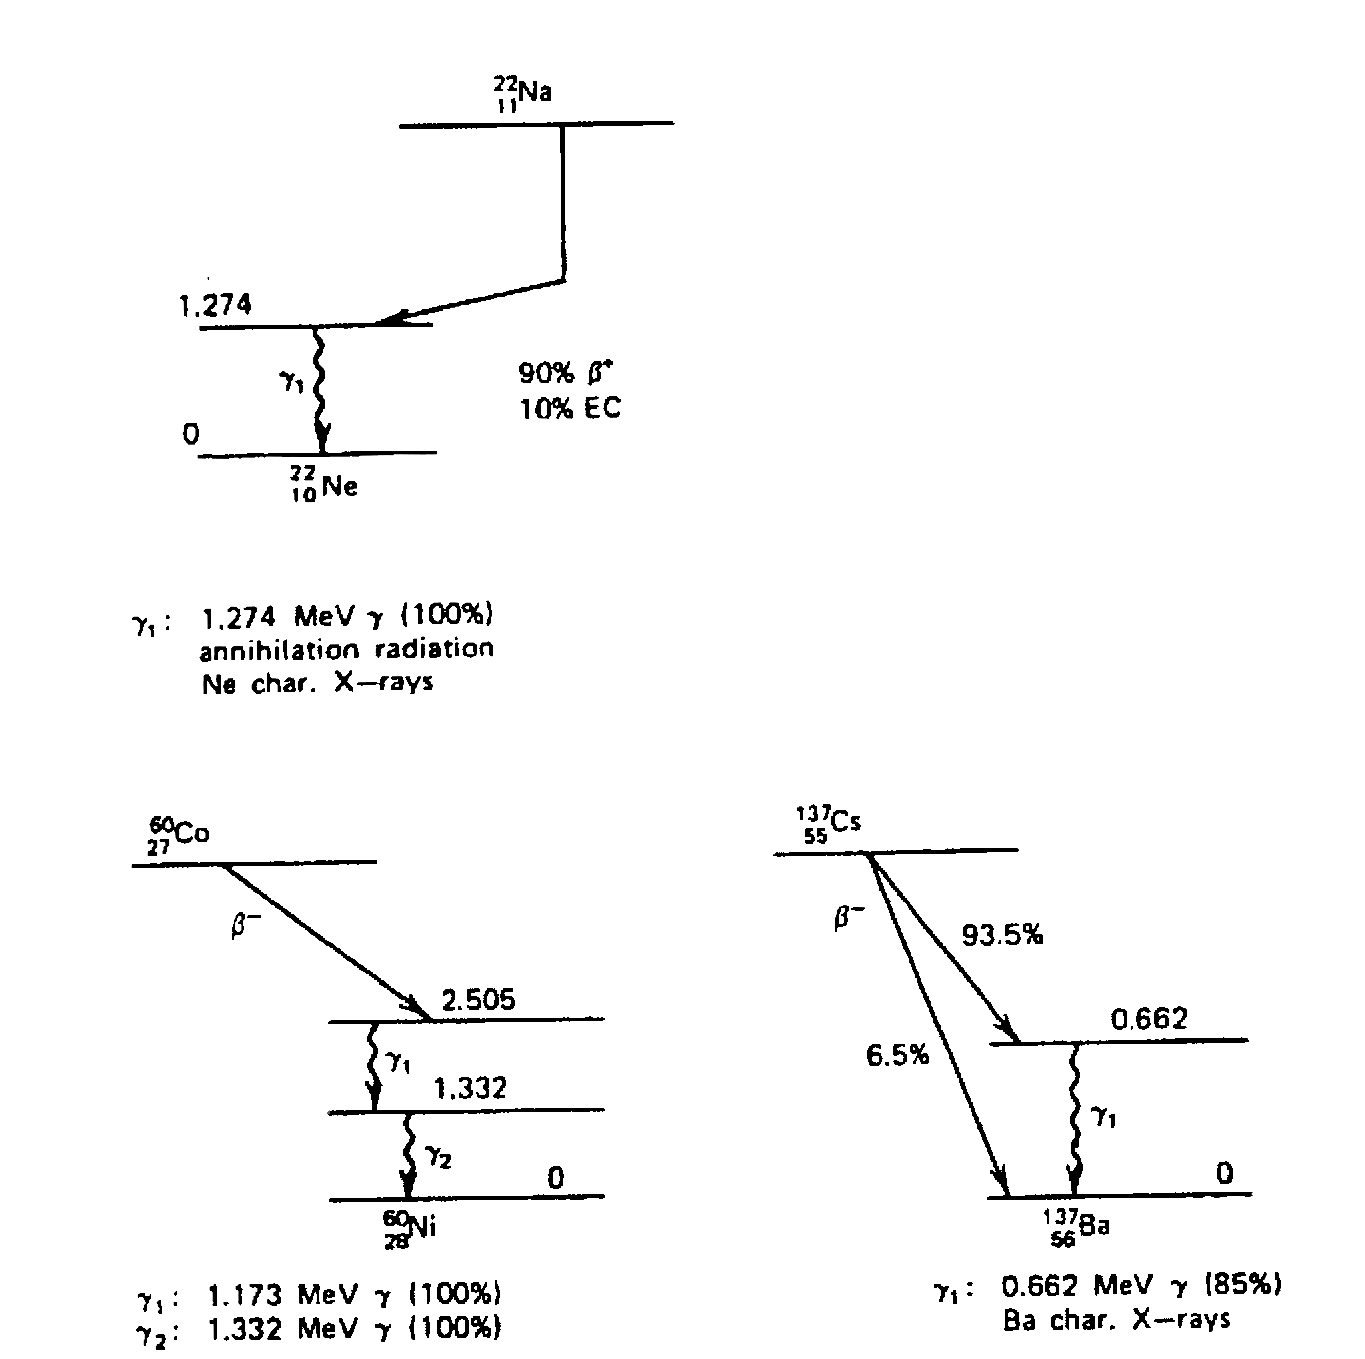
\includegraphics[width= 0.8 \linewidth]{charts/Zerfallsschematarot}
			\caption{
				Zerfallsschemata der relevanten Zerfälle. %TODO
				\cite{Anleitung}
			}
			\label{fig_zerfallsschemata}
	\end{figure}

	\subsection{Wechselwirkung mit Materie}
	% was ist die Schwierigkeit
	%TODO Comptonedge-Gedöns siehe der link?

	Die Detektion von $\gamma$-Strahlung ist dadurch gegenüber der Detektion von Strahlung aus anderen Zerfällen erschwert, als dass sie keine Ladung besitzt.
	Wenn man zusätzlich zum reinen Nachweis der Strahlung noch Information über Zeitpunkt des Auftreffens auf den Detektor, Intensität und Energie erhalten möchte, muss man sich mit der Wechselwirkung der Strahlung mit Materie auseinandersetzen und auf Basis dessen einen Detektor konstruieren.

	Da $\gamma$-Strahlung im Allgemeinen geringe Wechselwirkung mit Materie zeigt, muss für eine zielführende Messrate ein Stoff mit hoher Dichte (ein Festkörper) verwendet werden.

	\begin{figure}[H]
			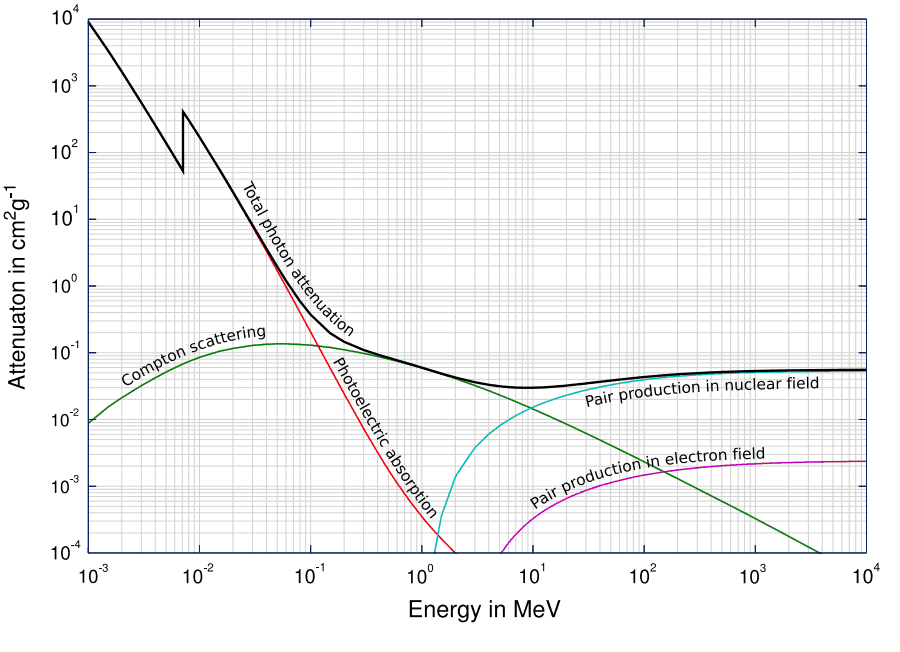
\includegraphics[width= 1 \linewidth]{charts/interaktion}
			\caption{
				Wirkungsquerschnitt von Photonen in Materie in Abhängigkeit von der Energie aufgeteilt in Compton-Effekt, photoelektrischen Effekt und Paarbildung sowie der Gesamtwirkungsquerschnitt.
				\cite{atomkraft}
			}
			\label{fig_wirkunsquerschnitt_gamma}
	\end{figure}

	In \cref{fig_wirkunsquerschnitt_gamma} ist der Wirkungsquerschnitt von Photonen in Materie durch die verschiedenen Effekte dargestellt.
	Außerdem steigt die Wechselwirkungwahrscheinlichkeit mit der Ladungszahl der Materie, durch die sich das Photon bewegt.

	% Abhängigkeit von Wirkungsquerschnitt von Energie? andere Faktoren?

	\subsubsection{Photoeffekt}
	% Vernachlässigung der Bindungsenergie `bei Photoeffekt möglich?
	% Abhängigkeit von Wirkungsquerschnitt von Energie für Photoeffekt?
	% warum sind da Stufen im Wirkungsquerschnitt?
	Beim Photoeffekt gibt ein $\gamma$-Photon seine Energie an ein Hüllenelektron im Detektor ab und wird dabei absorbiert.
	Das Hüllenelektron wird aus der Atomhülle gelöst, wofür Energie des Photons aufgewendet wird, und bewegt sich dann mit der Restenergie als kinetischer Energie durch die Materie.
	Die Energie der $\gamma$-Strahlung ($\ge \SI{100}{keV}$) ist dabei so deutlich größer als die Ionisierungsenergie (Größenordnung von wenigen \si{}{eV}), dass angenommen werden kann, dass alle Energie der $\gamma$-Strahlung in kinetische Energie umgesetzt wird.
	Für den Wirkungsquerschnitt gilt nach \cite{queensu}:

	\begin{equation}
		\label{eq_photo_wirk}
		\sigma \propto Z^5 E_\gamma^{-\frac{7}{2}}
	\end{equation}

	Außerdem hängt der Wirkungsquerschnitt in der $\gamma$-Energie von den Ionisationskanten ab, sodass eine Stufenform entsteht, da der Wirkungsquerschnitt ansteigt, wann immer die Ionisationsenergie einer weiteren Schale erreicht wird.

	\subsubsection{Comptoneffekt}

	Beim Comptoneffekt streut ein $\gamma$-Photon mit einem freien (oder quasi-freien) Elektron.
	Dabei ändern sich Energie und Bewegungsrichtung des Photons, da Energie auf das Elektron übertragen wird und eine Ablenkung stattfindet.
	Dies ist in \cref{fig_Compton} dargestellt.
	Der Energieübertrag auf das Elektron beträgt:
	\begin{equation}
		\label{eq_compton_energie}
		E_\text{e} = E_\gamma \left[ 1 - \frac{1}{1+(E_\gamma /M_\text{e} c^2)(1-\cos \varphi)} \right]
	\end{equation}

	Das Spektrum ist kontinuierlich, da in Abhängigkeit von der Geometrie des Stoßes ein beliebiger Anteil der Energie des Photons (bis zu einer Maximalenergie) an das Elektron übertragen werden kann.
	%TODO warum U-förmig?

	\begin{figure}[H]
			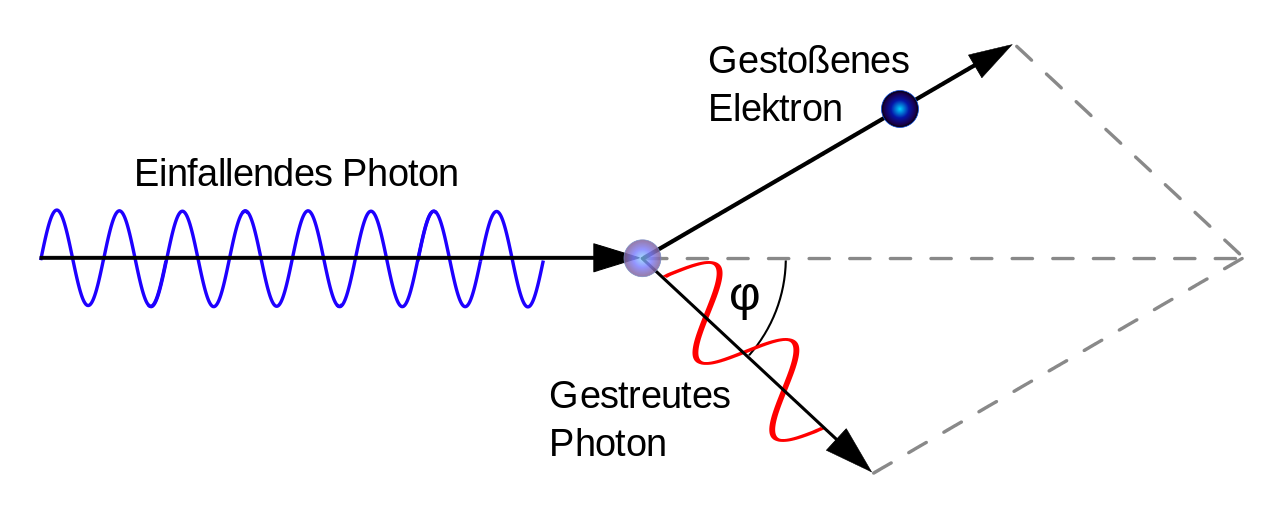
\includegraphics[width= 0.5 \linewidth]{charts/Comptonstreuung}
			\caption{
				Schematische Darstellung des Compton-Effekts.
				\cite{comptonwiki}
			}
			\label{fig_Compton}
	\end{figure}

	\subsubsection{Paarbildung}
	% waas ist für Paarbildung ötig?
	% Sekundäreffekte bei Paarbildung?
	In Wechselwirkung mit einem Atom (oder anderen Teilchen) kann ein $\gamma$-Photon die Entstehung eines Elektron-Positron-Paares hervorrufen.
	Dafür muss es mindestens die Ruheenergie des Teilchenpaares (\SI{1022}{keV}) besitzen.
	Das Photon wird dabei vernichtet und die überschüssige Energie geht in kinetische Energie der Reaktionsprodukte über.

	Das dabei entstandene Positron wird durch Wechselwirkung mit dem Rest der Probe unter Aussendung von Bremsstrahlung abgebremst.
	Wenn es ausreichend stark abgebremst ist, kann es mit einem Elektron in der Probe das instabile Positronium bilden.
	Beim Positronium unterscheidet man je nach Spinausrichtung von Positron und Elektron in Parapositronium ($S=0$) und Orthopositronium ($S=1$).
	Aufgrund von Spin- und Impulserhaltung zerfällt Orthopositronium in eine ungerade Anzahl Photonen, die mindestens \num{3} beträgt.
	Aus analogen Gründen zerfällt Parapositronium in eine gerade Anzahl Photonen, aber mindestens \num{2}.
	Da Zerfälle, die die Produktion einer geringeren Menge an Photonen voraussetzt, wahrscheinlicher sind, zerfällt Orthopositronium deutlich langsamer als Parapositronium.
	Gleichzeitig kann durch Umgebungswechselwirkung Orthopositronium in Parapositronium übergehen, was während der vergleichsweise langen Zerfallsdauer wahrscheinlich ist.
	Deswegen kann man sich in den folgenden Betrachtungen im Wesentlichen auf den Zerfall von Parapositronium in zwei Photonen mit einer Energie von \SI{511}{keV} beschränken.

	Positronium unterscheidet sich von Wasserstoff (ohne Neutron) dadurch, dass sich nicht ein Elektron im Coulombfeld des deutlich schwereren Protons befindet, sondern sich gleichschweres Positron und Elektron im gegenseitigen Einfluss befinden.
	Auch beim Wasserstoff unterscheidet man in Ortho- und Parawasserstoff.
	% Positronium-Gedöns: Vorraussetzungen
	% Vergleich zu Wasserstoff
	% Warum ist Zerfall in zwei am wahrscheinlichsten?

	\subsection{Gamma-Spektrum}
	% Welche Einflüsse?
	%TODO Was passiert bei Zerfällen mit mehreren Gamma-Linien?
	%TODO welche anderen Effekte kann man sehen?
	%TODO Spektren vorhersagen: 22Na, 60Co, 137Cs

		In \cref{fig_Gammaspektrum} ist ein idealisiertes Gammaspektrum dargestellt.
		Wenn das Photon im Spektrum Paarbildung verursacht und beide Photonen, die beim Zerfall des Positroniums entstehen, gemessen werden, bildet sich dies im so genannten Full Energy Peak ab, der bei der Energie des ursprünglichen $\gamma$-Photons liegt.
		Wenn jedoch eins oder beide der Photonen aus dem Positronium den Detektor verlassen, ohne nachgewiesen zu werden, misst man eine um \SI{511}{keV} bzw. \SI{1022}{keV} verringerte Energie.
		Der kontinuierliche Untergrund ergibt sich durch den Comptoneffekt, wobei die maximale Energie durch die Comptonkante bezeichnet wird.
		Dazu tritt der Backscatteruntergrund, der durch Comptoneffekte außerhalb des Absorbers entsteht, bei denen die gestreuten Photonen dann im Detektor nachgewiesen werden.
		Der Photoeffekt führt zur Messung der Photolinie, die dem Full Energy Peak entspricht.

		\begin{figure}[H]
				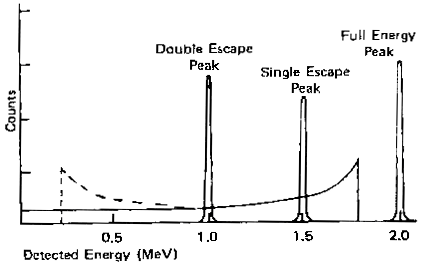
\includegraphics[width= 0.75 \linewidth]{charts/Spektrumschema}
				\caption{
					Schematische Darstellung des Compton- (durchgezogen) und Rückstreu-Effekts (gestrichelt).
					\cite{Anleitung}
				}
				\label{fig_Gammaspektrum}
		\end{figure}


	\subsection{Gamma-Detektoren}

	\subsubsection{Halbleiterdetektoren}
	% pn-Übergang? als gamma-detektor?
	% Problem herstellung von "pure semiconductor"
	%TODO Was ist wichtig bei Verwendung von Halbleiterdetektor?
	% Warum muss der gekühlt werden?
	%TODO Was braucht man sonst noch?
	% Warum Schicht undotierte Schicht?-> breitere RLZ
	%TODO Unterschiede Szintallator und Halbleiter

	Der Übergang zwischen p- und n-dotiertem Halbleiter wird als pn-Übergang bezeichnet.
	Durch die überschüssigen bzw. fehlenden Elektronen im Gitter und den folgenden Ladungsfluss, bei dem Elektronen und Löcher rekombinieren, entsteht im pn-Übergang eine Raumladungszone.
	Diese ist räumlich begrenzt, da der Rekombination das Coulombfeld der verschobenen Ladungen gegenübersteht.

	Wenn ein Photon auf das Halbleitermaterial trifft, entsteht ein Elektron-Loch-Paar.
	Elektron und Loch können sich durch den Halbleiter bewegen und, wenn sie sich treffen, rekombinieren.
	Wenn sie jedoch durch das elektrische Feld einer äußeren Hochspannung getrennt werden, können sie nachgewiesen werden.
	Für diese Art der Detektion muss der Halbleiter extrem rein sein, da sonst durch Verunreinigungen Blindströme entstehen, die die Messung mit Rauschen überlagern können.
	Alternativ kann ein p-n-Übergang verwendet werden, der in Sperrrichtung gepolt ist.
	Durch das Feld in der Raumladungszone werden die Paare getrennt, bevor sie an Fehlstellen rekombinieren können.
	Um die Raumladungszone zu verbreitern, wird zwischen p- und n-dotierte Schicht eine Schicht intrinsischen Halbleiters gebracht.
	Dies nennt man pin-Diode.
	Ein solcher Detektor wird mit Stickstoff gekühlt, um das Rauschen zu reduzieren, da die Fermi-Energie der Elektronen mit der Temperatur steigt und bei höheren Temperaturen durch die Fermi-Dirak-Statistik der besetzten Zustände Elektronen ins Leitungsband angeregt werden können.
	Solche Elektronen können Rauschen verursachen.
	Bei geringen Temperaturen wird die Zustandsbesetzung aber schärfer und solche Effekte minimiert.

	\subsubsection{Szintillationsdetektor} % (von woanders klaubar)
	% welche gibt es, was sind die Unterschiede?
	% warum dotiert?

	% Auswahlkriterien für Szintillator für Gamma-Spektroskopie
	Ein Szintillator ist ein Detektor, der einfallende Strahlung in eine einfacher messbare elektromagnetische Strahlung umwandelt.
	Bei anorganischen Halbleiter-Szintillatoren wird durch die einfallende Strahlung ein Elektron aus den Valenzband in das Leitungsband angeregt und lässt im Valenzband ein Loch zurück.
	Wenn das Elektron an einer Störstelle mit dem Loch rekombiniert, kann dies durch die an der Störstelle modifizierten Bandstruktur schrittweise geschehen, weshalb Strahlung einer geringeren, leichter detektierbaren Wellenlänge frei wird.
	Um solche Störstellen hervorzurufen, kann das Material dotiert werden.
	Bei organischen Szintillatoren werden stattdessen Anregungen in Molekülen ausgenutzt, die bei der Abregung Photonen anderer Energien freiwerden lassen.

	Bei der Auswahl eines Szintillators sind folgende Punkte wichtig:

	\begin{enumerate}
		\item Transparenz für erzeugtes Licht
		\item hohe Effizienz: viele der einfallenden Photonen werden umgewandelt
		\item Antwortzeit: Verzögerung zwischen eintreffendem Photon und messbaren Photonen
		\item Linearer Zusammenhang zwischen Signal und Energie des einfallenden Photons
		\item geringe Anstiegs- und Abfallzeit des Signals
		\item Brechungsindex in der Nähe von Glas, um einen verlustfreien Anschluss an einen Photomultiplier zu erlauben
	\end{enumerate}

	\subsubsection{Photomultiplier}

	In einem Photomultiplier werden einzelne einfallende Photonen in ein messbares Signal umgewandelt.
	Das Funktionsprinzip ist in \cref{fig_Photomultiplier} dargestellt.
	Dabei löst zunächst ein einfallendes Photon an der Kathode (negative Spannung) ein Elektron aus.
	Dieses Elektron wird in Richtung der Anode (positive Spannung) beschleunigt und schlägt auf dem Weg dorthin aus den Dynoden zusätzliche Elektronen heraus.
	An der Anode kommen dann ausreichend viele Elektronen an, um einen messbaren Rückfluss zur Kathode zu erzeugen (bzw. über einen Widerstand eine messbare Spannung).

	\begin{figure}[H]
			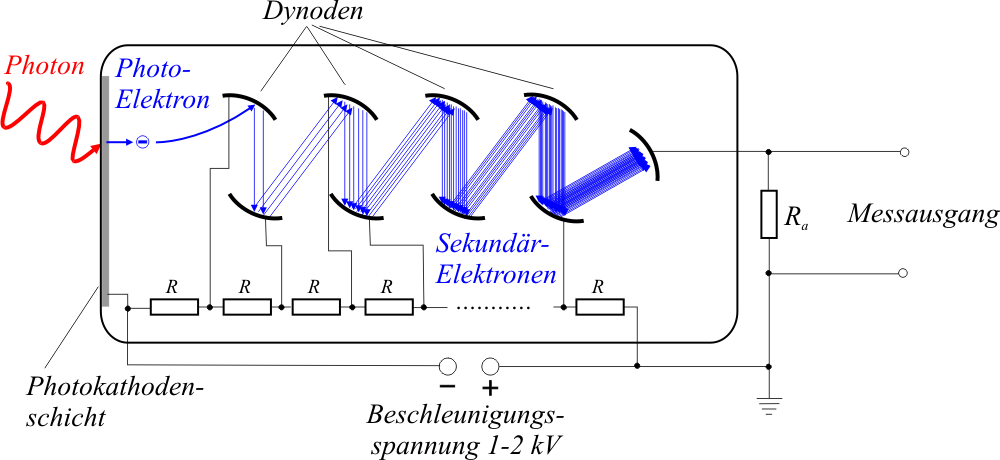
\includegraphics[width=0.6\linewidth]{charts/Photomultiplier}
			\caption{
			Schematische Darstellung eines Photomultipliers.
			\cite{Photomultiplier}
			}
			\label{fig_Photomultiplier}
	\end{figure}

	\subsection{Energieauflösung und mittlere Ionisationsenergie}
	Die Energieauflösung ist
	\begin{equation}
		\Delta E = \frac{\sigma(E)}{E},
	\end{equation}
	wobei $\sigma$ die Standardunsicherheit und $E$ die Position eines Peaks ist.

	Außerdem setzt sich die Energie aus der Ereignisanzahl und der mittleren Ionisationsenergie zusammen
	\begin{equation}
		\label{eq_eni}
		E=N I
	\end{equation}
	und
	\begin{align}
		\frac{\sigma(E)}{E} &= \frac{\sigma(N) I}{N I}= \frac{\sigma(N)}{N} \\
		&= \frac{\sqrt{N}}{N} = \frac{1}{\sqrt{N}}.
	\end{align}
	Es wurde verwendet das die Standardunsicherheit $\sigma(E)=\sigma(N)I$ ist, da $I$ als im Mittel konstant angenommen wird und da man von einer Poissonverteilung ausgehen kann ist $\sigma(N)=\sqrt{N}$.
	Somit folgt $N = \left(\frac{E}{\sigma}\right)^2$.
	Woraus sich mit \cref{eq_eni}
	\begin{equation}
		I = \frac{\sigma^2}{E}
	\end{equation}
	ergibt.

	\section{Methoden}
	% Bilder von der Website klauen
	% einer will Präsens
	% verwendete Proben
	% Wahl des Verstärkungsfaktors (pro Detektor gleich gelassen) -> so, dass alle Peaks im Spektrum sind durch kurzzeitmessung
	% Messdauern?
	% Erzprobe
% Photomultiplier? Was braucht man da sonst noch?->Lichtleiter, Vorverstärker.

	Es wird ein thallium-aktivierter Natrium-Iodid-Kristall (NaI(TI)) als Szintillationsdetektor und  ein lithium-kompensierter Germanium-Halbleiterdetektor (Ge(Li)) verwendet, um $\gamma$-Spektren verschiedener Quellen zu messen.
	Die verwendeten Proben sind: $^{22}$Na, $^{137}$Cs, $^{60}$Co, eine aus vielen Isotopen gemischte Probe und eine Probe aus einem unbekannten Erz.

	Der Szintillationsdetektor wird mit Stickstoff gekühlt.
	Der Szintillator ist möglichst verlustfrei mit dem Photomultiplier verbunden (ähnliche Brechungsindizes von Szintillator, Kleber und Eingangsfenster des Photomultipliers).
	Damit das Signal über Koaxialkabel übertragen werden kann, wird es bei beiden Detektoren vorverstärkt.
	Dann wird es im Hauptverstärker verstärkt und über einen Multichannel Analyzer in Energiekanälen gesammelt und digitalisiert.
	Die Verstärkung wird jeweils so gewählt, dass die zur Verfügung stehenden Kanäle möglichst vollständig ausgenutzt werden und alle relevanten Peaks sichtbar sind.
	Für die Detektoren wird die Verstärkung aber jeweils gleich gehalten, damit eine Kalibrierung anhand einer Probe möglich ist.

	Es wird je nach Aktivität der Probe etwa \SIrange{10}{60}{\minute} gemessen.
	Die Probe wird außerdem je nach Probe in unterschiedlichem Abstand zum Detektor positioniert, wobei die Signalrate ausreichend gering gehalten wird, sodass die Totzeit unter \SI{15}{\percent} liegt und die Signalrate für die Proben etwa gleich ist.

	\subsection{Kalibrierung}
	% Warum Na-22 zur Kalibrierung?
	%TODO wie beeinflusst die Kalibrierunsicherheit die späteren Messungen?
	%TODO Was bestimmt Peakbreite?
	%TODO Warum misst man die Breite?->Zusammenhang zu
	%TODO Definition FWHM, Sigma
	%TODO kann man hier Kalibrierunsicherheit vernachlässigen?

	Es wird $^{22}$Na zur Kalibrierung verwendet, da hier beim Beta-Plus-Zerfall Positronen frei werden, die die Bildung von Positronium und die Entstehung von Photonen bei \SI{511}{keV} verursachen.
	Gleichzeitig entstehen, wie in\cref{fig_zerfallsschemata} zu erkennen ist, Photonen bei \SI{1274}{MeV}.
	Diese beiden Energien liegen recht weit auseinander und ergeben so gut Peaks, um anhand ihnen die Kanalzahl in eine Energie zu übersetzen.

	Die Peakbreite ergibt sich aus der verwendeten Elektronik und der Unsicherheit des Detektors, wobei angenommen werden kann, dass letztere dominiert.
	Man kann die Peakbreite verwenden, um das Auflösungsvermögen der Detektoren zu bestimmen.
	Die Standardunsicherheit ist durch die Breite des Peaks auf halber Höhe (FWHM) gegeben als: $\sigma = \frac{\text{FWHM}}{2\sqrt{2 \ln 2}}$

	\section{Ergebnisse und Diskussion}
	%TODO Unsicherheiten


	\subsection{Beobachtung und Datenanalyse}
	% Allgemeine Beobachtungen
	% Einflüsse von veränderten Parametern auf Messung

	\subsubsection{Unsicherheiten}
	Alle Unsicherheiten werden nach GUM bestimmt und berechnet.
	Für diese Berechnungen wurde die Python Bibliothek \enquote{uncertainties} herangezogen, welche den Richtlinien des GUM folgt.
	Die Fits verwenden die Methode der kleinsten Quadrate, außer wenn anders angegeben.
	Die Unsicherheit der gemessenen Ereignisse $N$ ist durch $\sqrt{N}$ gemäß Poisson-Verteilung gegeben.
	\subsubsection{Modell}
	Die aufgenommenen Spektren der $^{22}$Na-Probe sind in \cref{fg_Na_ch} abgebildet.
	Es wurden bei jeder Messung die ersten 95 Kanäle vernachlässigt, da all diese nahe Null Ereignisse liefern und die Erstellung ein physikalischen Modells des Spektrums im Randbereich unmöglich machen. %TODO schönerer Satz wäre schöner
	Das Modell wurde in \enquote{Fityk} aus Gaußkurven zusammengesetzt.
	\begin{figure}[H]
		\centering
		\begin{subfigure}[c]{\textwidth}
			\centering
			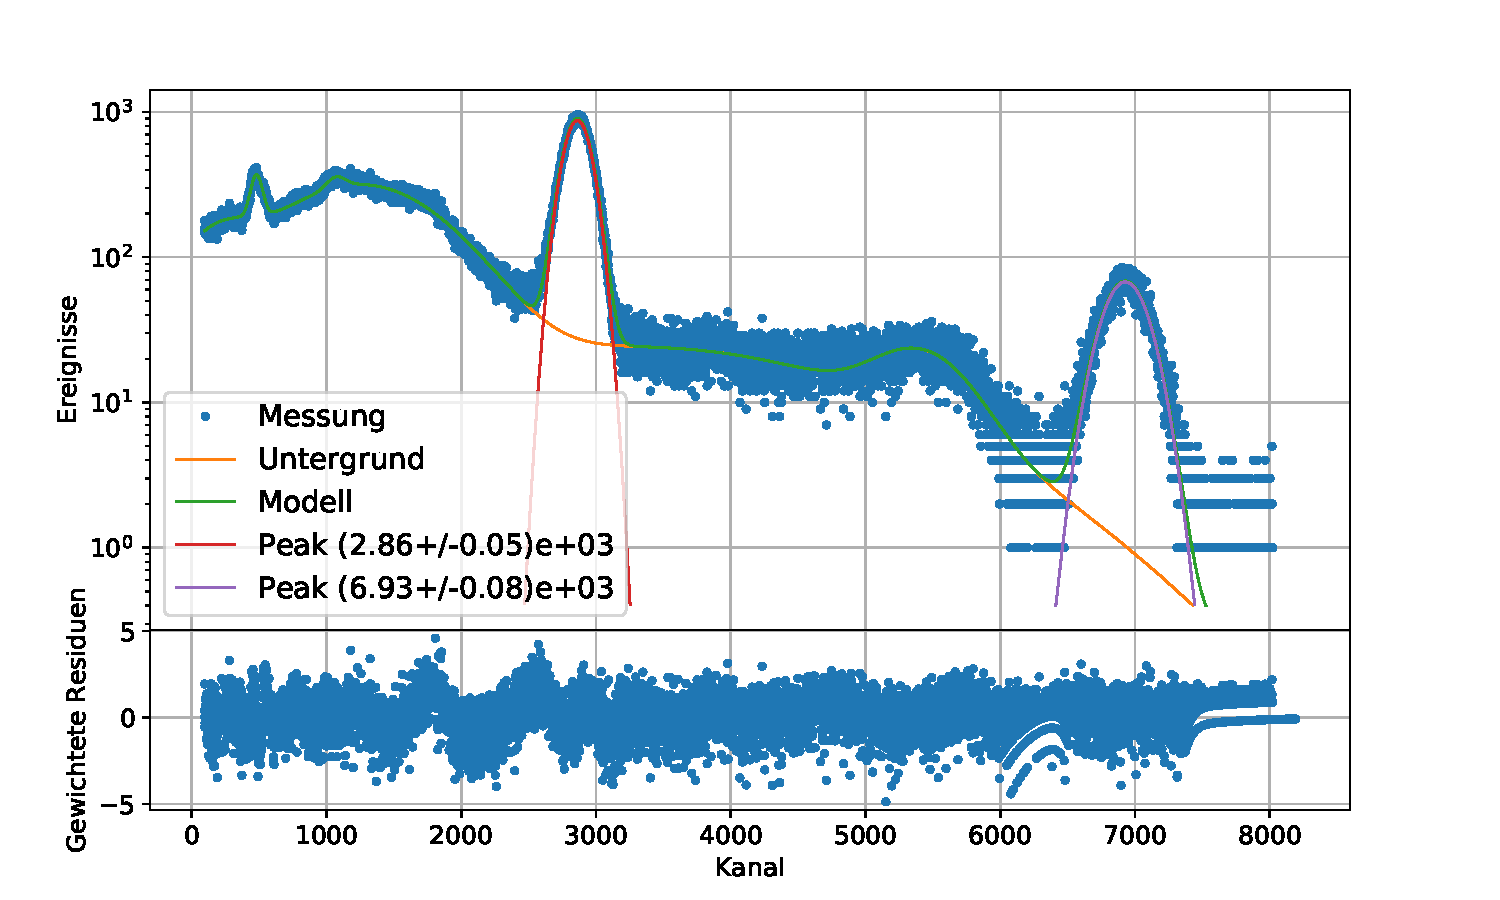
\includegraphics[width= 1 \linewidth]{img/NaNaCh.pdf}
			\subcaption{
				NaI-Detektor.
			}
		\end{subfigure}
		\begin{subfigure}[c]{\textwidth}
			\centering
			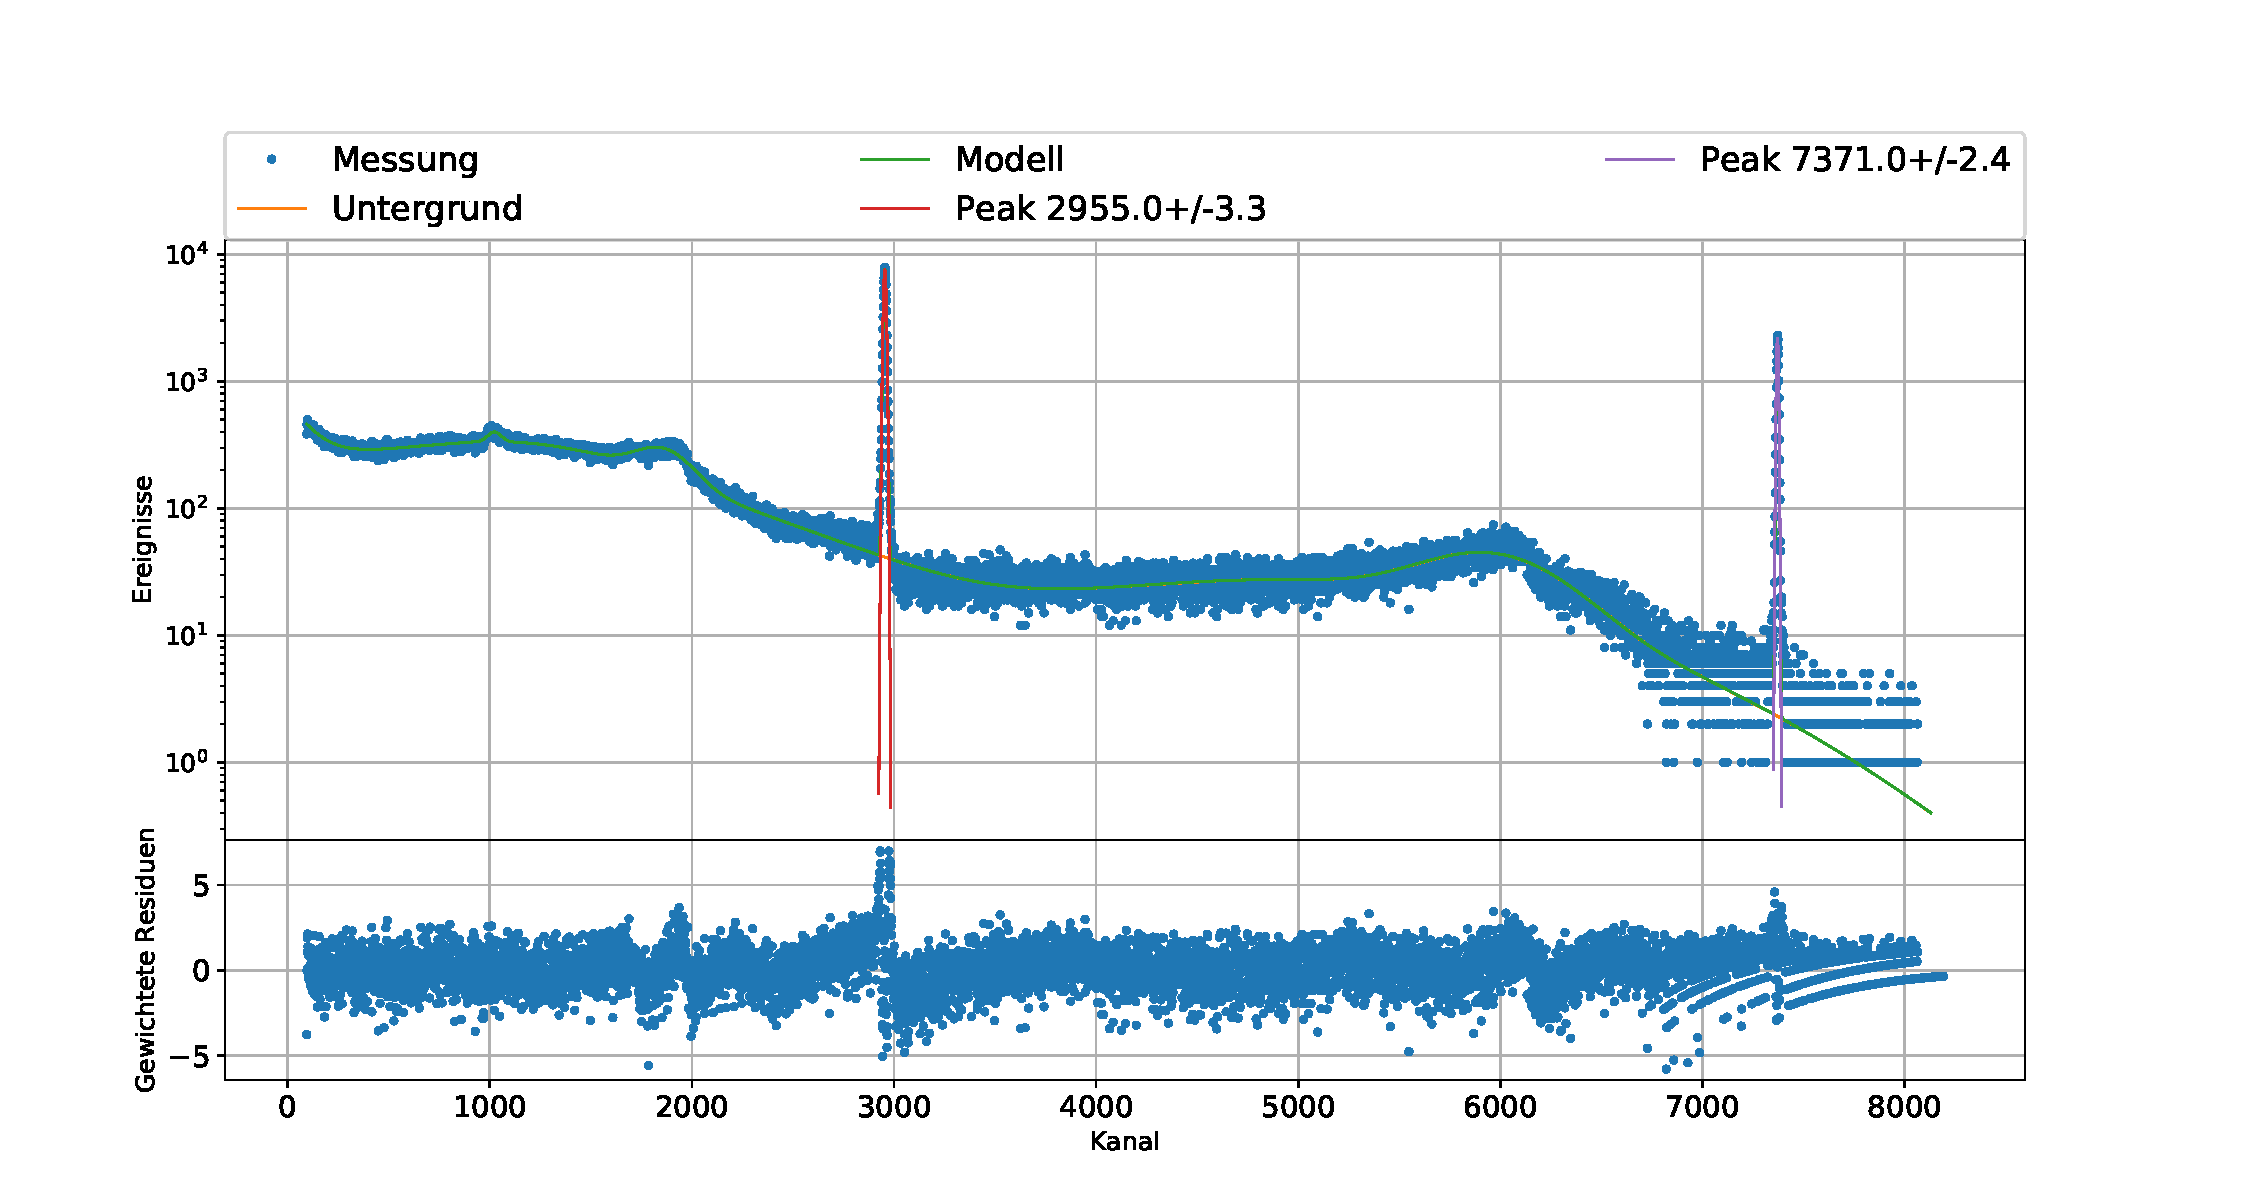
\includegraphics[width= 1 \linewidth]{img/NaGeCh.pdf}
			\subcaption{
				Ge-Detektor.
			}
		\end{subfigure}
		\caption{$^{22}$Na-Probe}
		\label{fg_Na_ch}
	\end{figure}


	\subsubsection{Kalibration}
  Mittels der Literaturwerte der Peaks der $^{22}$Na-Probe (\SI{511}{keV} und \SI{1274}{keV} \cite{Anleitung}) lassen sich die Kanäle umrechnen zu einer Energieskala.  %TODO erläutert in Theorie?
	In \cref{fg_kali_mix} sind in blau (gelb) die zwei Kalibrationspunkte für den NaI-Detektor (Ge-Detektor) abgebildet.
	Die Unsicherheit des Kanals ist durch die Standardunsicherheit der Gaußkurve in \cref{fg_Na_ch} gegeben.

	\begin{figure}[H]
			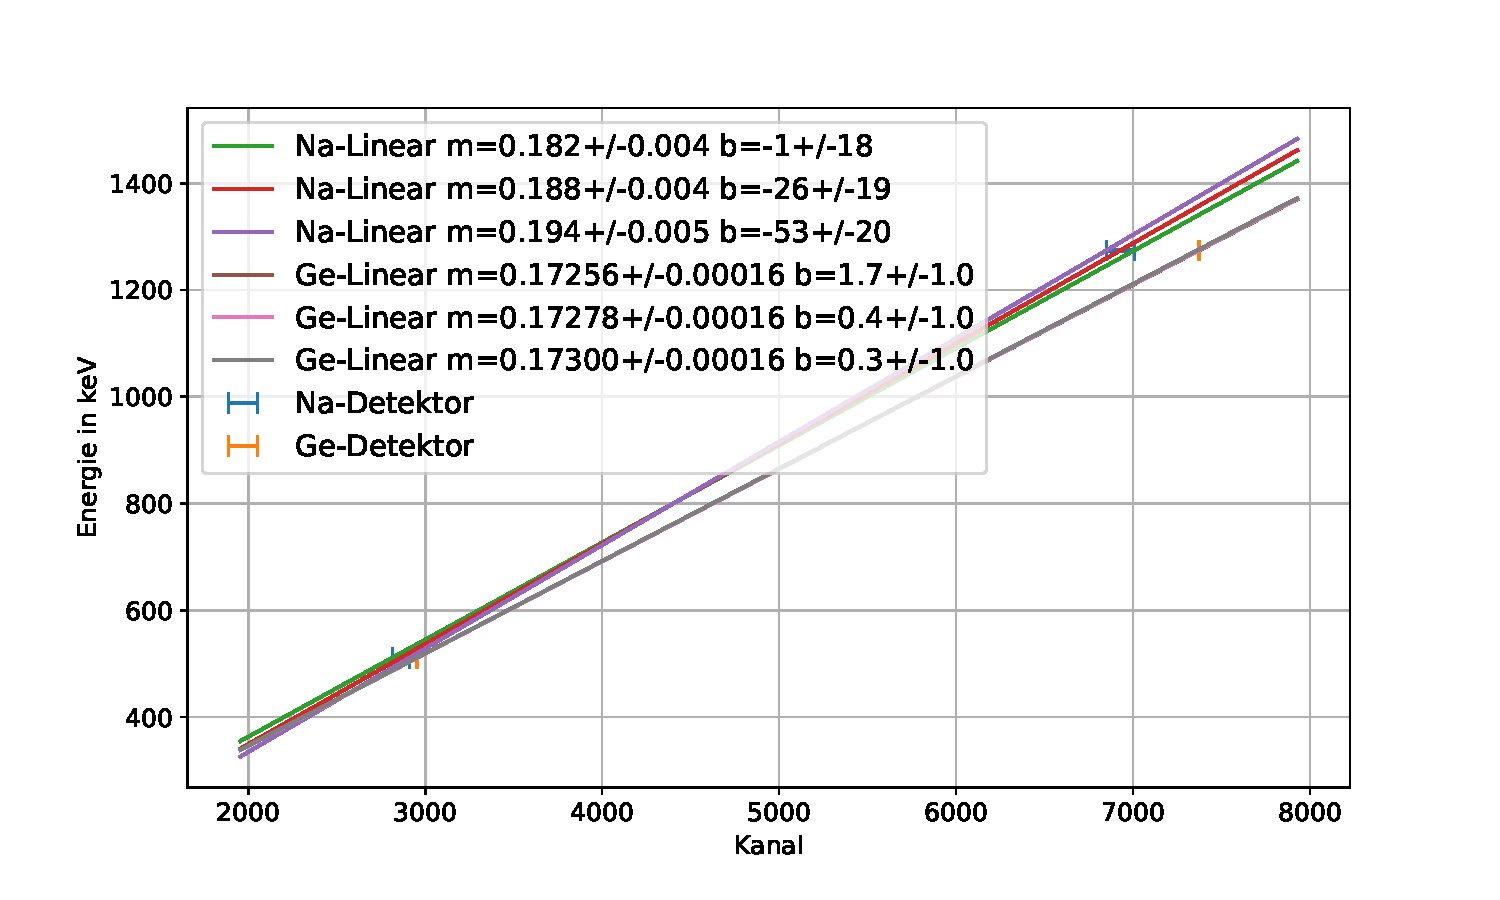
\includegraphics[width= 0.8 \linewidth]{img/kali_mix.pdf}
			\caption{
				Kalibrationsgeraden $f(x)=mx+b$.
				$m$ ist die Steigung der Gerade in \si{keV}.
				$b$ ist der y-Achsenabschnitt in \si{keV}.
			}
			\label{fg_kali_mix}
	\end{figure}

	Da ein linearer Fit zwischen zwei Punkten mit Unsicherheiten mit dem \enquote{Least-Square-Fit} nicht zielführend ist, werden drei Geraden durch die Messintervalle gelegt, sodass sich eine mittlere, maximale und minimale Steigung ergeben. %TODO hier wird er wissen wollen, warum der nicht zielführend ist.
	Eine Mittelung dieser Werte ist in \cref{tb_kali_avg} aufgeführt.

\begin{table}[H]
		\centering
		\begin{tabular}{c | c | c  }
			 Detektor& $m$ in \si{keV}& $b$ in \si{keV} \\ \hline
			 NaI & \SI{0.188+-0.015}{} & \SI{-30+-60}{} \\
			 Ge & \SI{0.1728+-0.0006}{} & \SI{1.3+-2.3}{} \\
		\end{tabular}
		\caption{
		Gemittelte Kalibrationsparameter für NaJ- und Ge-Detektor.
		}
		\label{tb_kali_avg}
\end{table}
%TODO y-Achse ist ca. Null, nice, aber diskutieren warum Anfang alles Null?
Damit lässt sich ein Kanal $c$ nach \cref{eq_trans} in die Energie $E$ transformieren.
\begin{equation}
	\label{eq_trans}
	E = m\cdot c + b
\end{equation}

\subsubsection{Diskussion}

Wie bereits in \cref{fg_Na_ch} zu erkennen ist, misst der Ge-Detektor deutlich schmalere Peaks, hat also eine bessere Auflösung.
Dies spiegelt sich auch in einer größeren Unsicherheit im Kalibrationsparameter des NaI-Detektors wieder.
Die y-Achsenabschnitte der Kalibrierungsgeraden haben alle die Null im Fehlerintervall, weshalb hier kein Widerspruch zur erwarteten näherungsweisen Linearität des Szintillators (bzw. Halbleiterdetektor) gesehen werden kann.

\subsection{Peaks und Kanten}
In \crefrange{fg_Na}{fg_Mix} sind die kalibrierten Spektren von vier Proben für jeden der Detektoren dargestellt.
Die horizontalen Linien, die sich im höher energetischen Bereich ergeben, entstehen durch die logarithmischen Darstellung.

%TODO In der Theorie?
Die Comptonkante berechnet sich aus dem Literaturwert $E_\gamma$ für einen Full-Energy-Peak ($\varphi=\SI{180}{\degree}$ in \cref{eq_compton_energie}):
\begin{equation}
	E_C = E_\gamma - \frac{E_\gamma }{1+2E_\gamma/m_ec^2}
\end{equation}
Die Rückstreukante lässt sich analog mit:
\begin{equation}
	E_R =  \frac{E_\gamma}{1+2E_\gamma/m_ec^2}
\end{equation}
bestimmen.
Die Literaturwert stammen aus \cref{tb_lit_peaks}.
	Die Zusammensetzung der Mischprobe ist nicht bekannt, jedoch lassen sich die Peaks ziemlich genau Kernübergängen zuordnen.
	Anhand derer Literaturwerte lassen sich somit auch Compton- und Rückstreukante berechnen.
Außerdem wurden die Ränder des Bereichs der Röntgenfluoreszenz von Blei gekennzeichnet (aus \cite{XRAYDB}).

\begin{table}[H]
		\centering
		\begin{tabular}{c | c | c | c | c | c}
			 Isotop& $^{60}$Co & $^{137}$Cs& $^{22}$Na & $^{241}$Am & $^{109}$Cd \\ \hline
			 $E_\gamma$ in \si{keV} & \SI{1332}{}&\SI{662}{}& \SI{1274}{} &\SI{60}{}&\SI{88}{} \\
			 & \SI{1173}{} &&\SI{511}{}& \\
		\end{tabular}
		\caption{
		Literaturwerte für Full-Energy-Peaks.\cite{Anleitung}
		}
		\label{tb_lit_peaks}
\end{table}

%TODO caption ? Unsicherheit?
\begin{figure}[H]
		\centering
		\begin{subfigure}[c]{\textwidth}
			\centering
			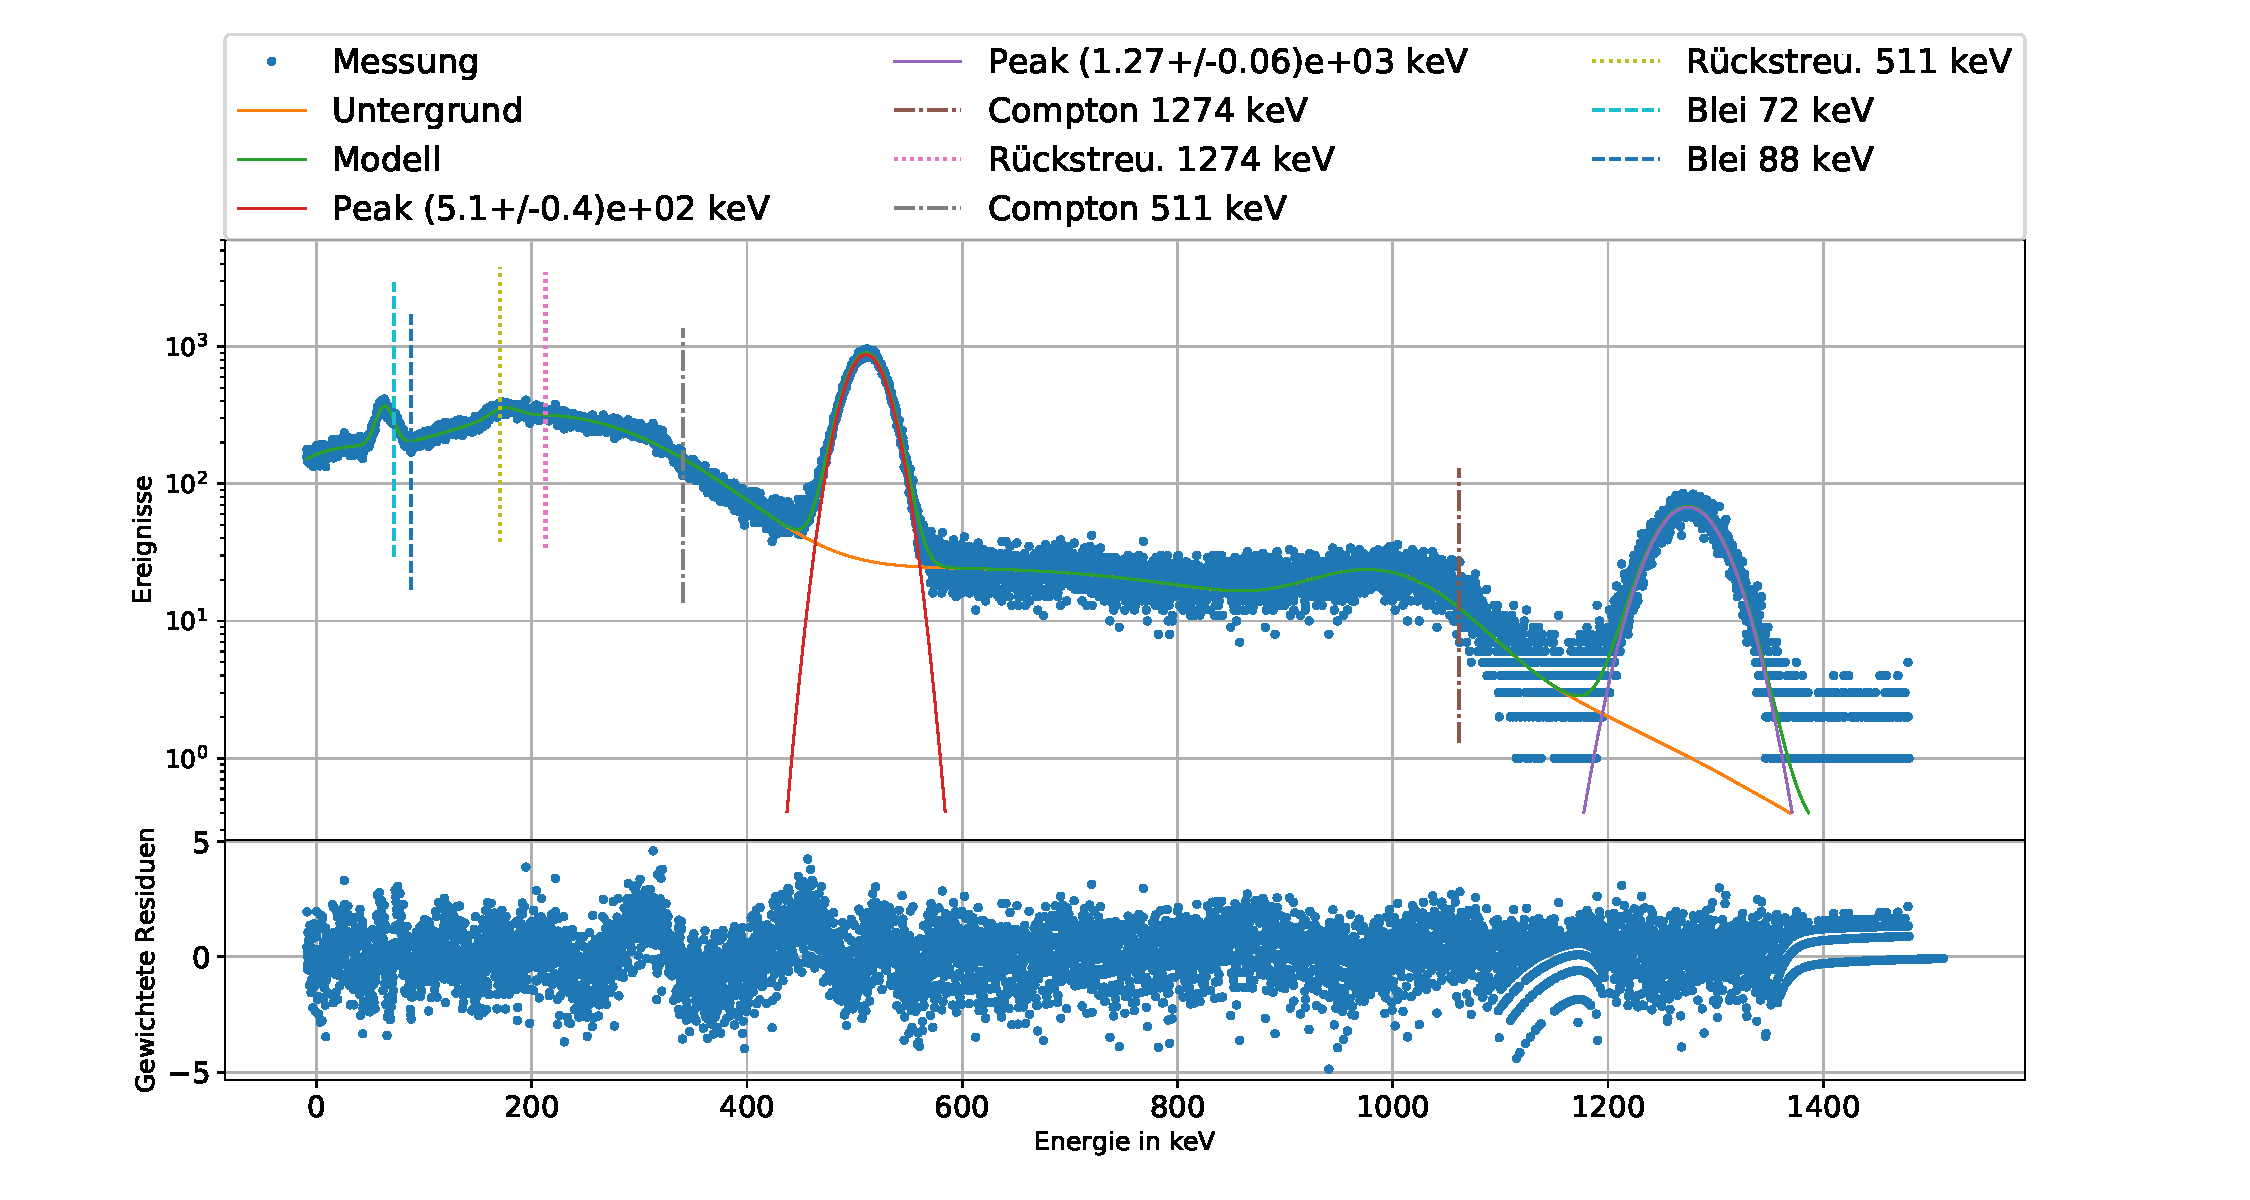
\includegraphics[width= 1 \linewidth]{img/NaNa.pdf}
			\subcaption{
				NaI-Detektor.
			}
		\end{subfigure}
		\begin{subfigure}[c]{\textwidth}
			\centering
			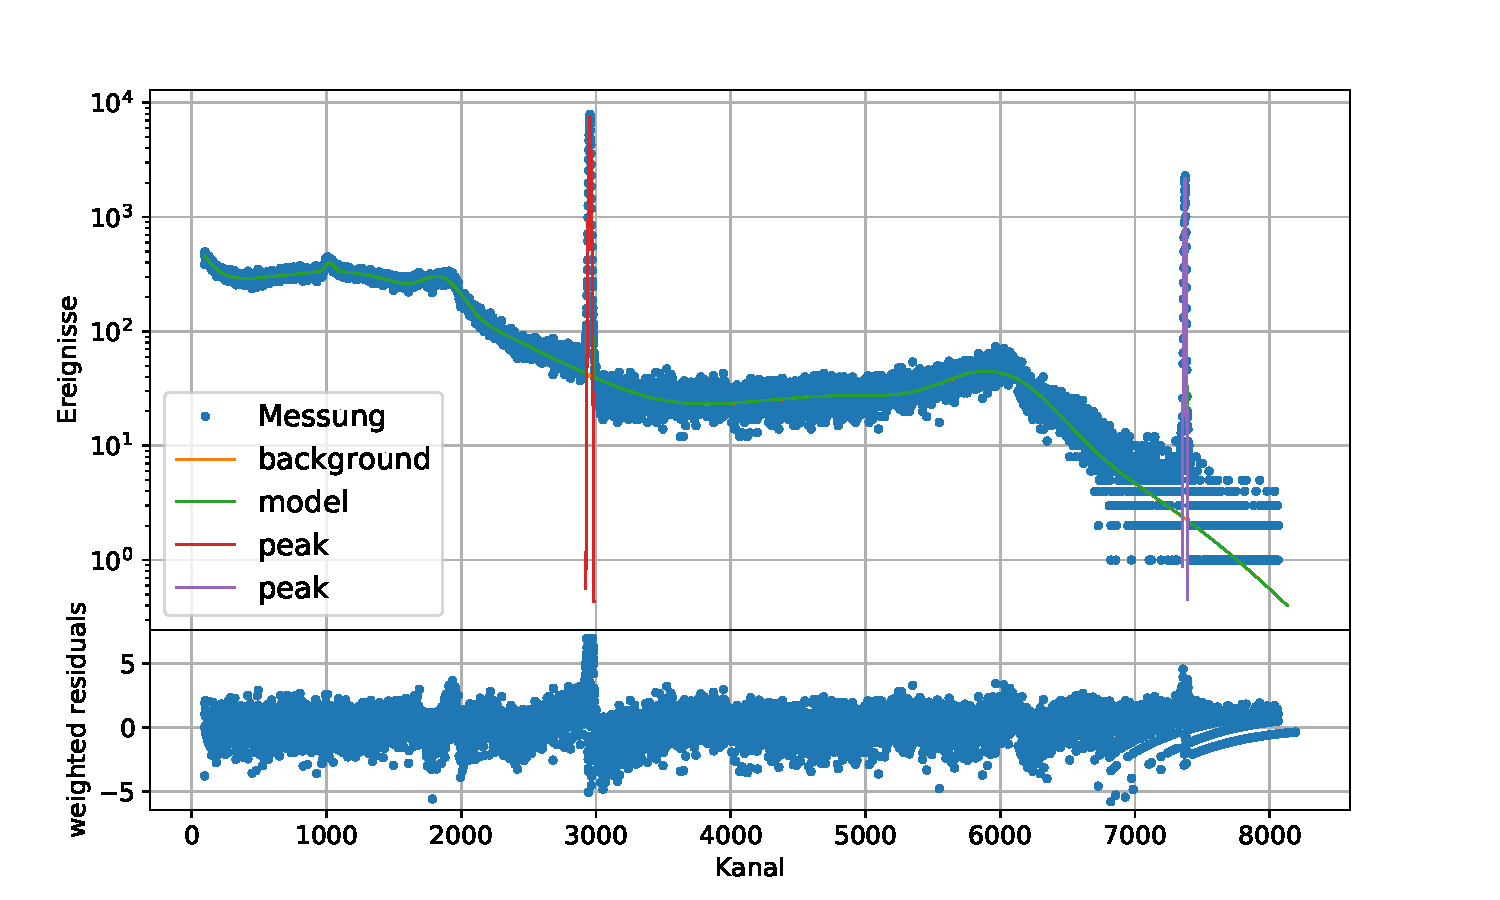
\includegraphics[width= 1 \linewidth]{img/NaGe.pdf}
			\subcaption{
				Ge-Detektor.
			}
		\end{subfigure}
		\caption{$^{22}$Na-Probe}
		\label{fg_Na}
	\end{figure}


\begin{figure}[H]
		\centering
		\begin{subfigure}[c]{\textwidth}
			\centering
			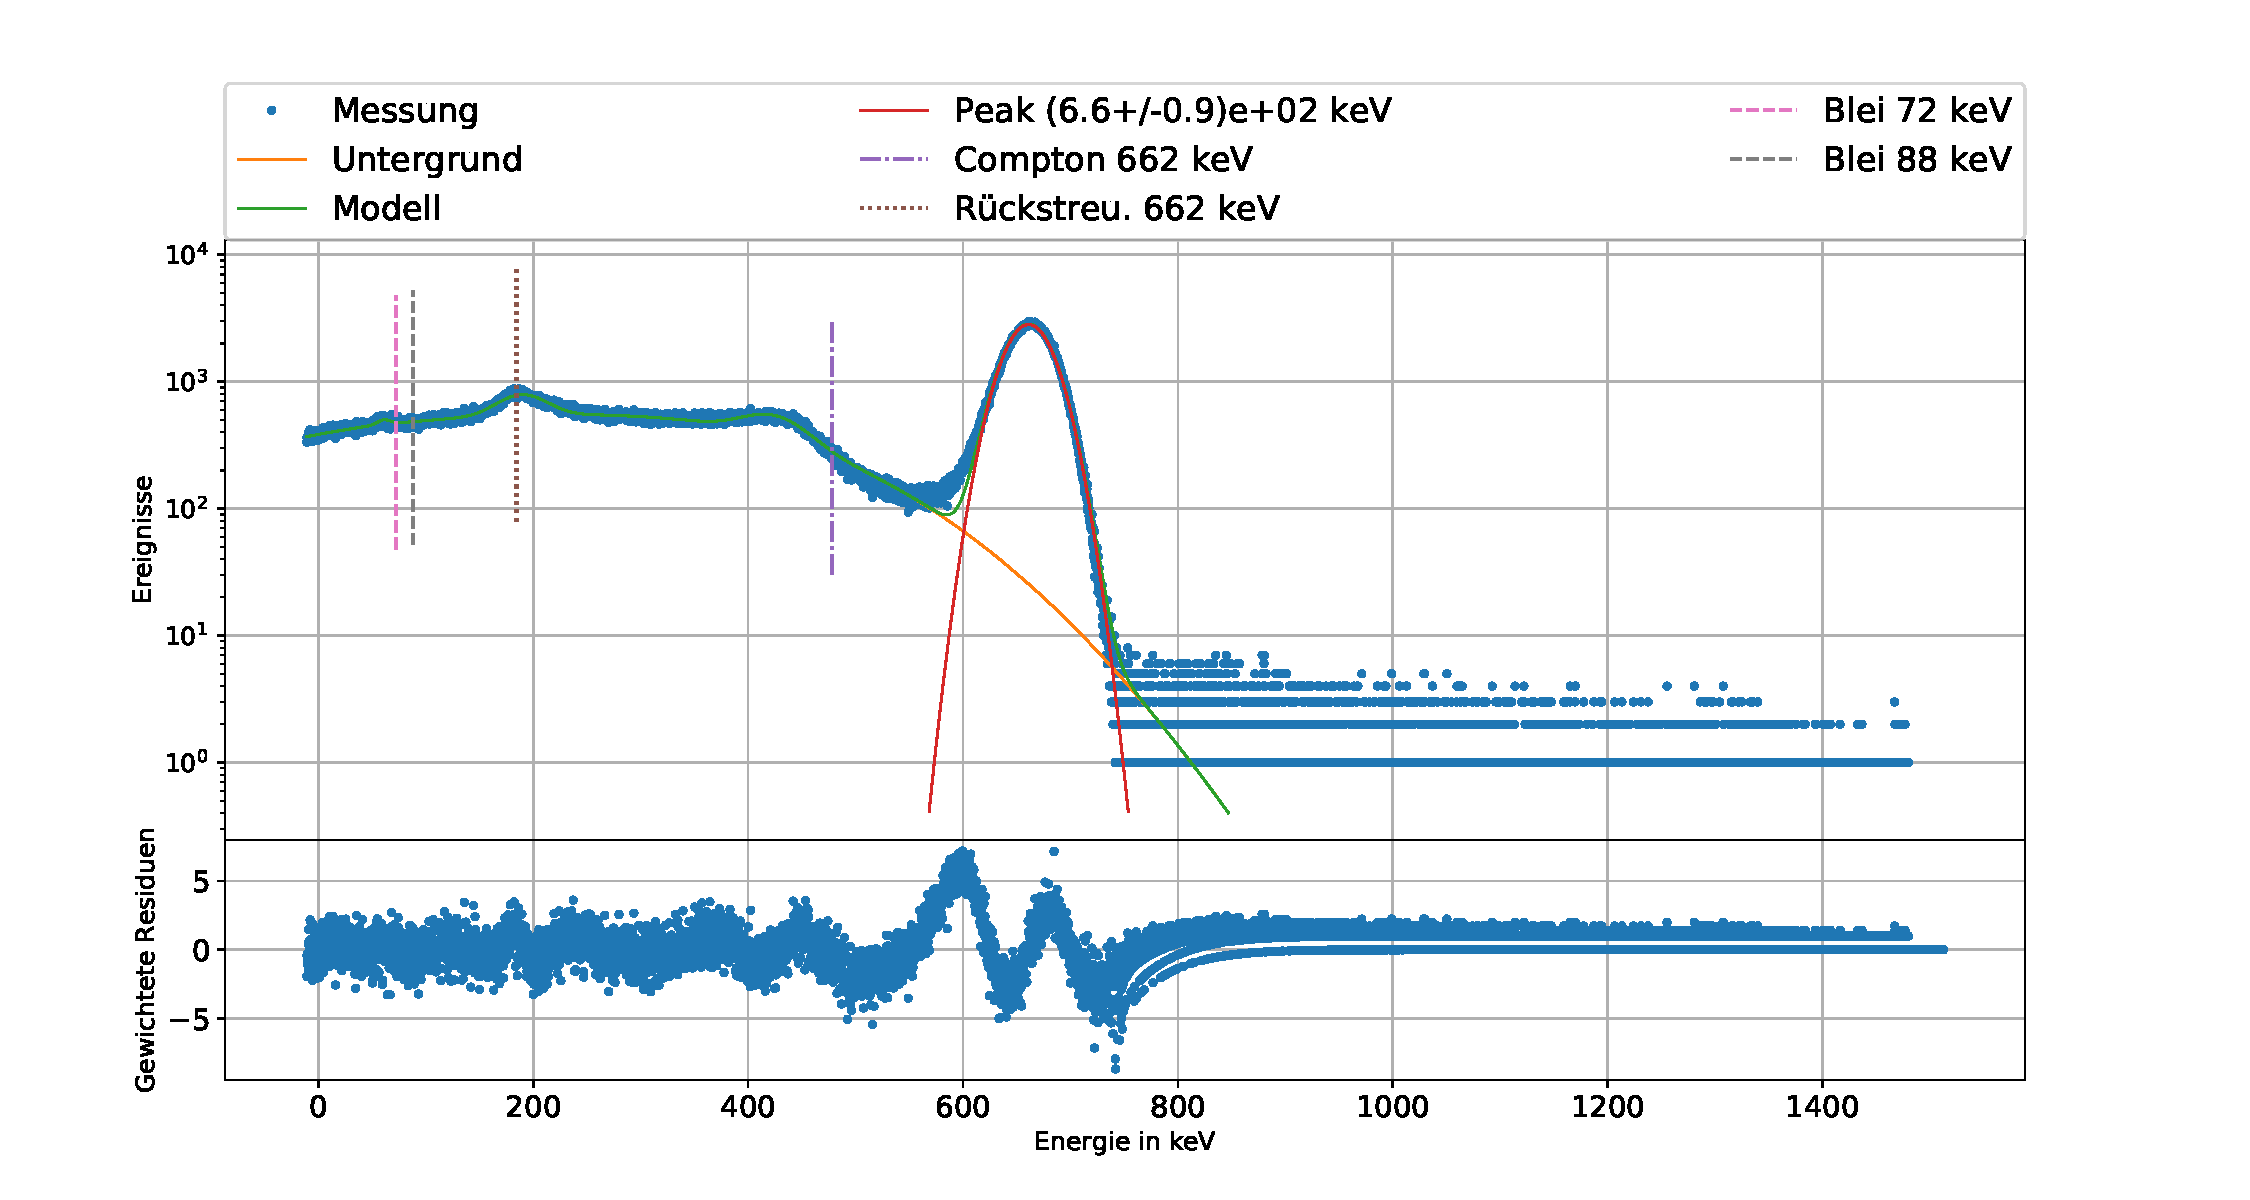
\includegraphics[width= 1 \linewidth]{img/CsNa.pdf}
			\subcaption{
				NaI-Detektor.
			}
		\end{subfigure}
		\begin{subfigure}[c]{\textwidth}
			\centering
			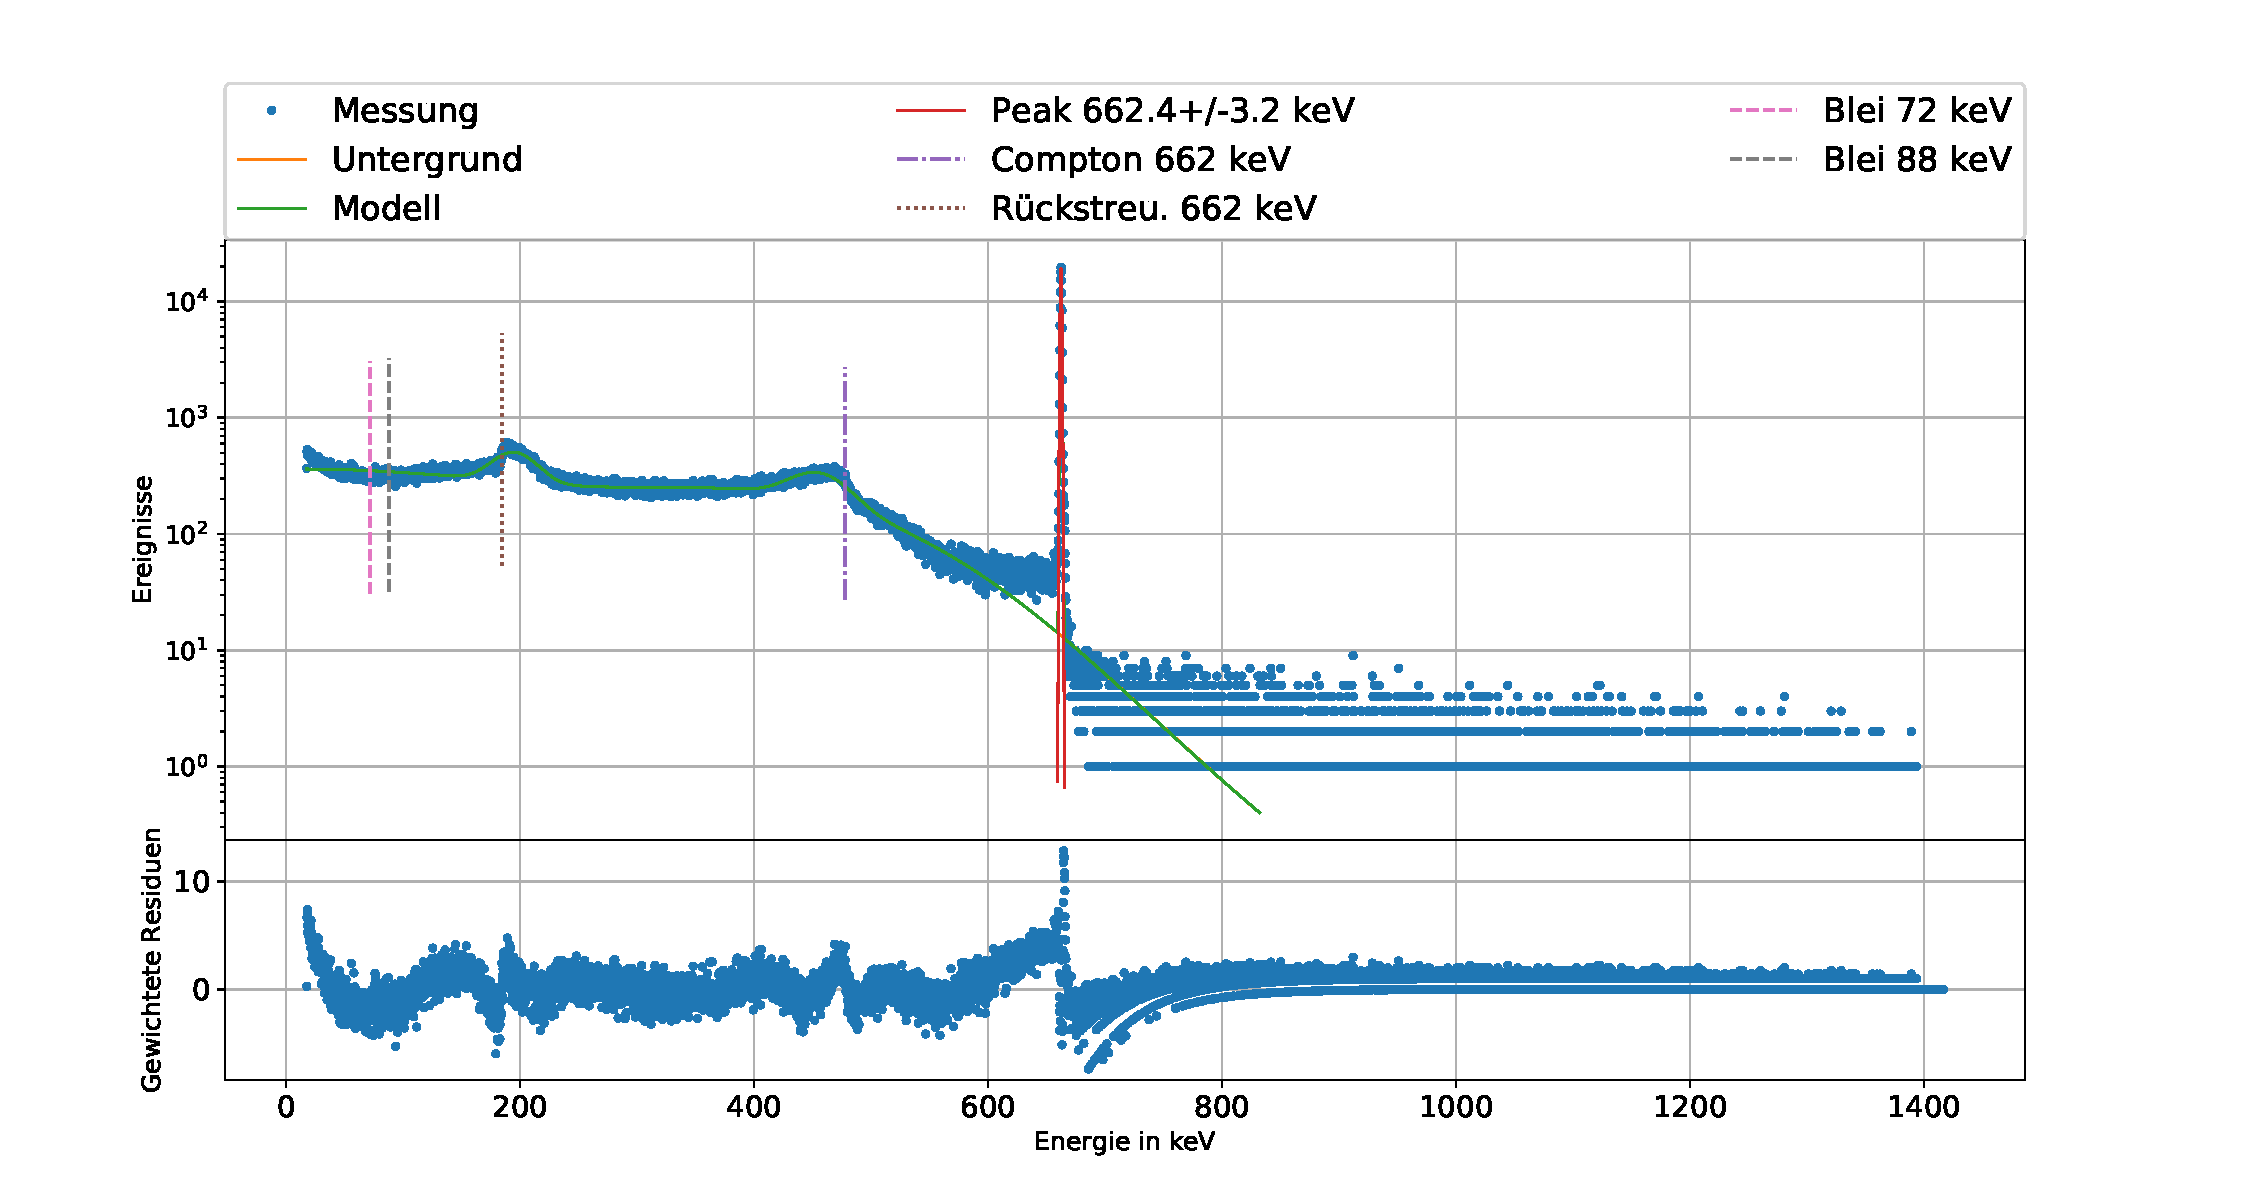
\includegraphics[width= 1 \linewidth]{img/CsGe.pdf}
			\subcaption{
				Ge-Detektor.
			}
		\end{subfigure}
		\caption{$^{137}$Cs-Probe}
		\label{fg_Cs}
	\end{figure}

\begin{figure}[H]
		\centering
		\begin{subfigure}[c]{\textwidth}
			\centering
			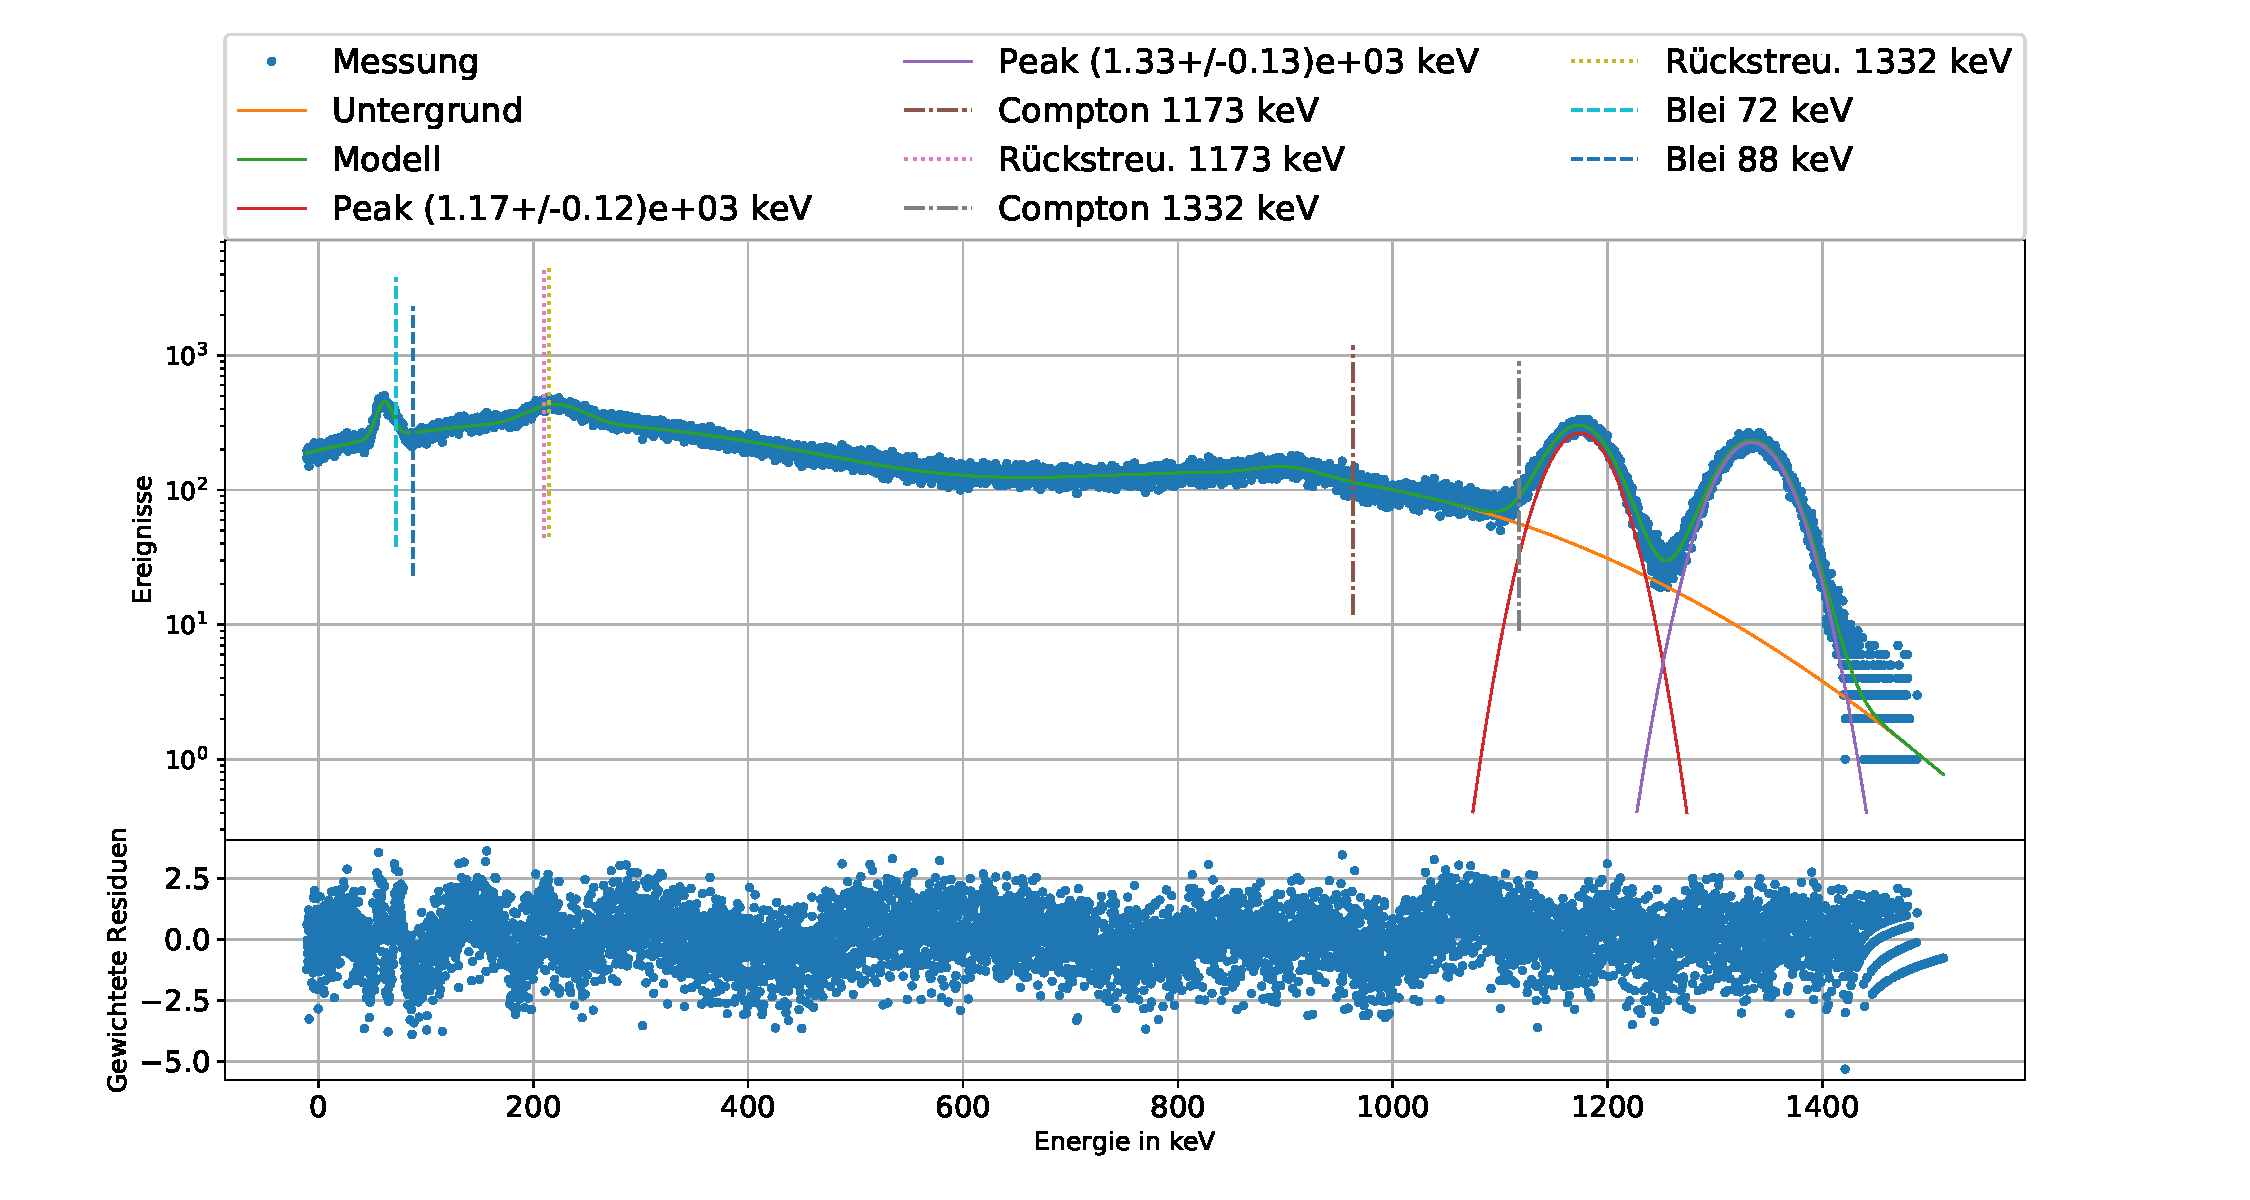
\includegraphics[width= 1 \linewidth]{img/CoNa.pdf}
			\subcaption{
				NaI-Detektor.
			}
		\end{subfigure}
		\begin{subfigure}[c]{\textwidth}
			\centering
			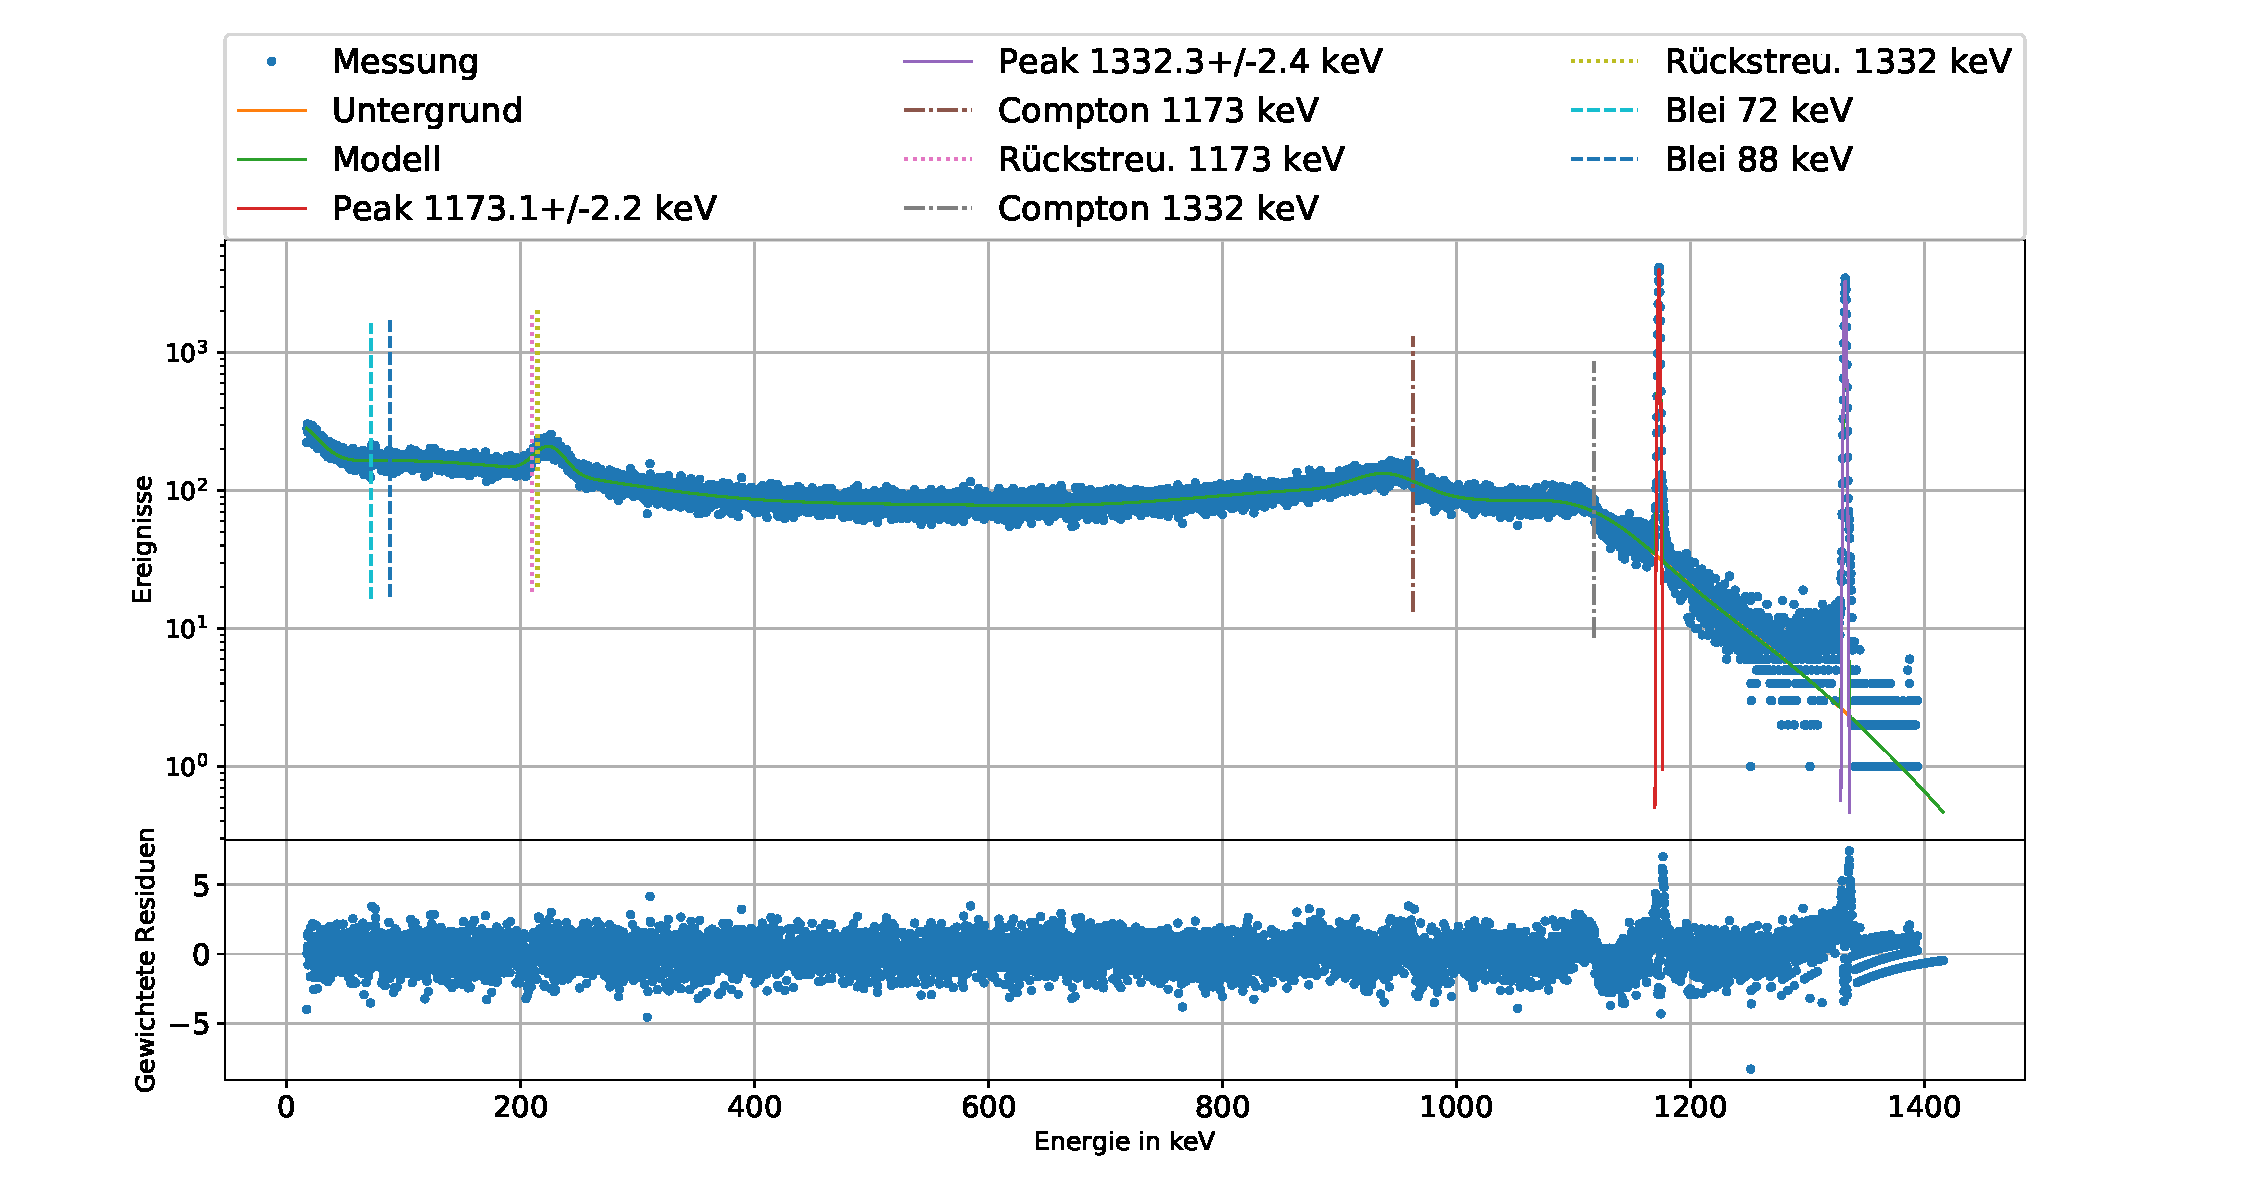
\includegraphics[width= 1 \linewidth]{img/CoGe.pdf}
			\subcaption{
				Ge-Detektor.
			}
		\end{subfigure}
		\caption{$^{60}$Co-Probe}
		\label{fg_Co}
	\end{figure}

\begin{figure}[H]
		\centering
		\begin{subfigure}[c]{\textwidth}
			\centering
			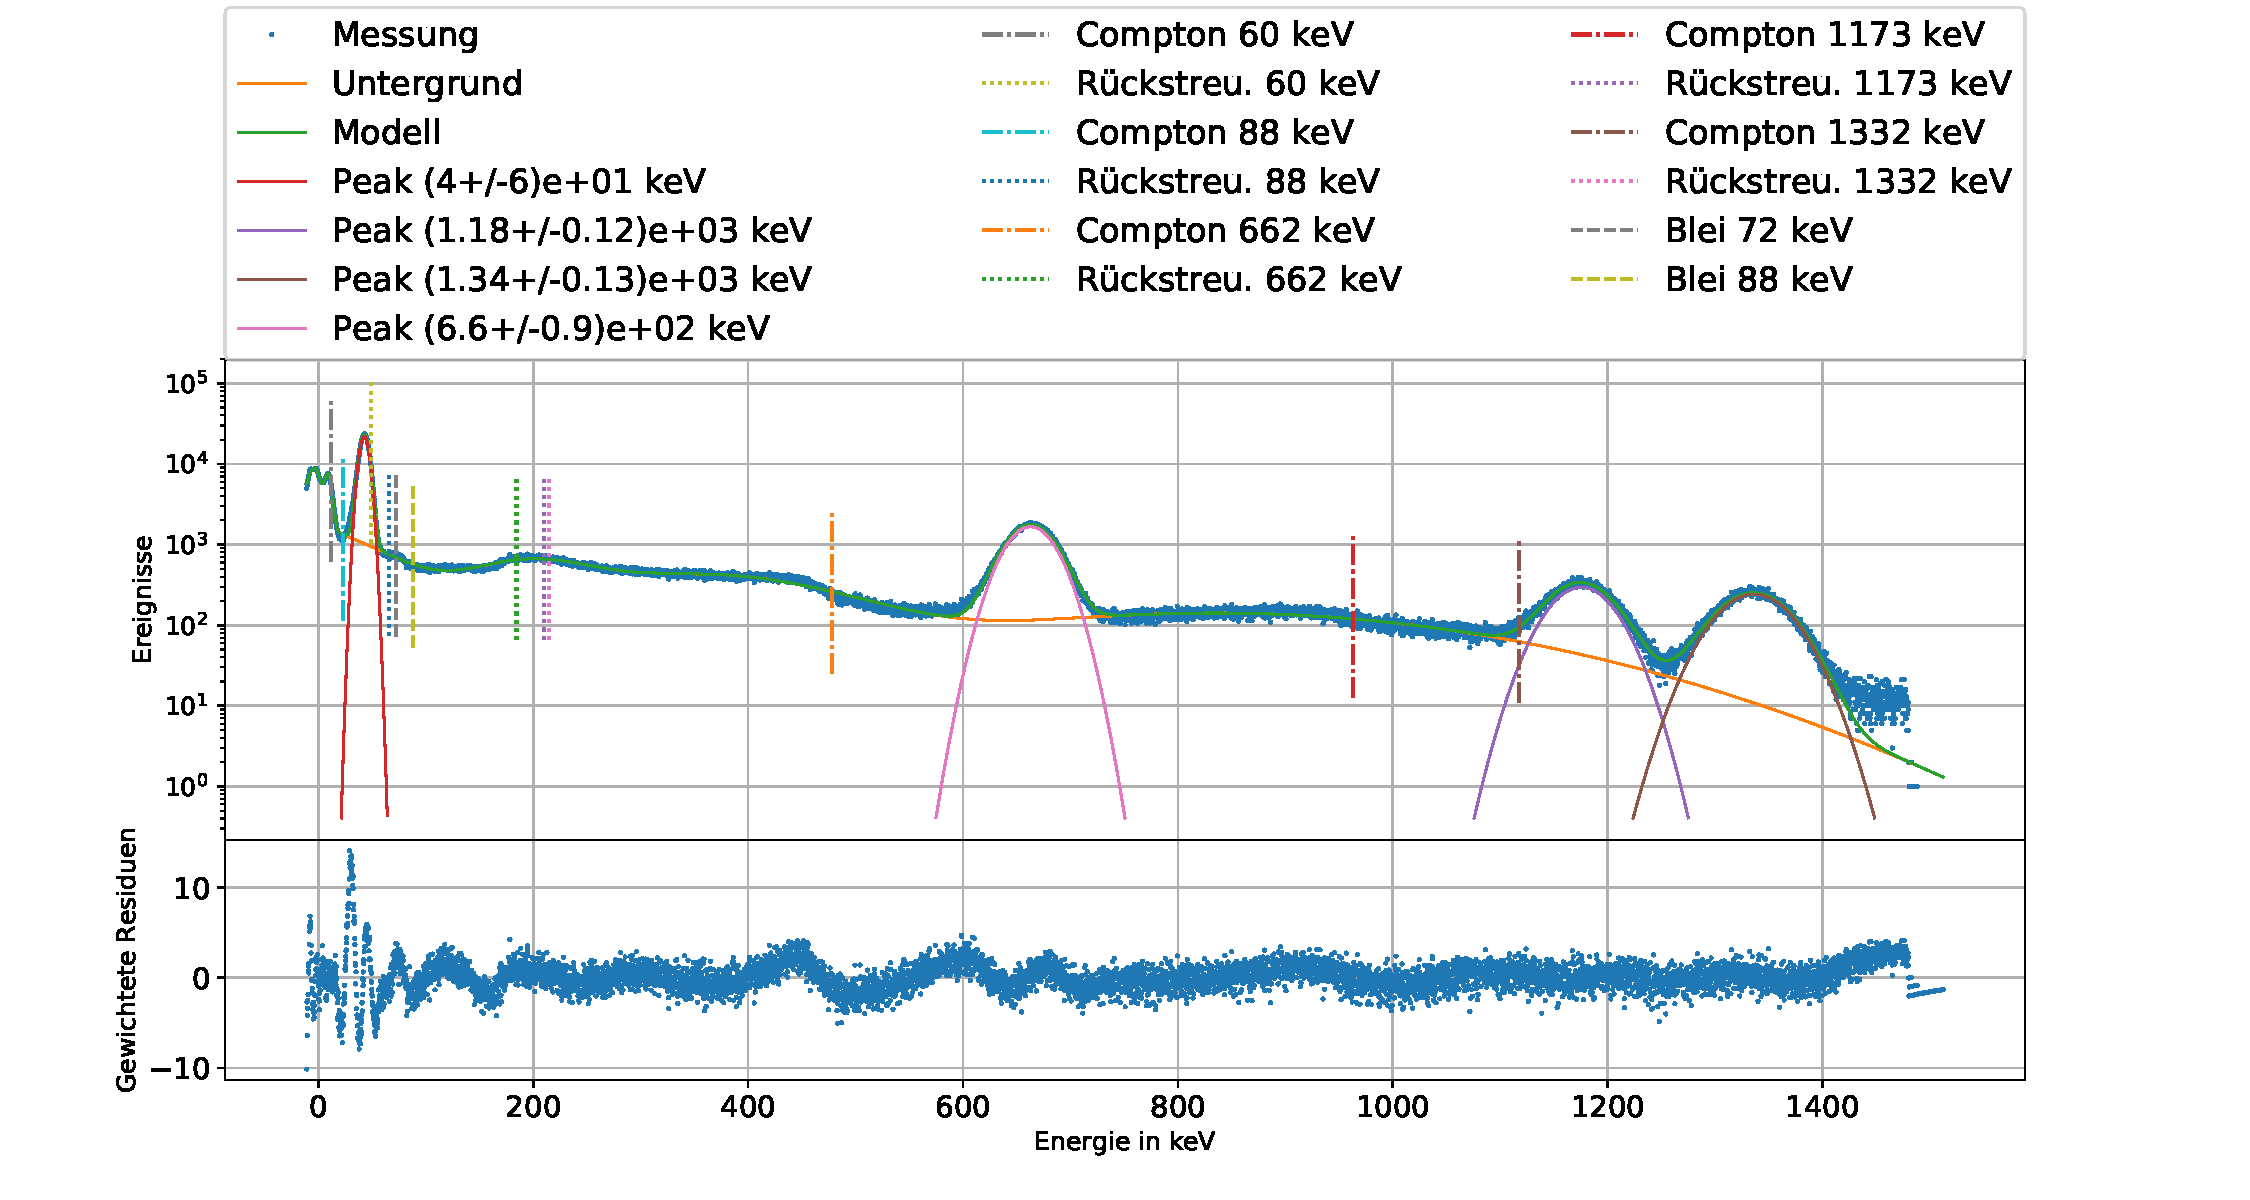
\includegraphics[width= 1 \linewidth]{img/MixNa.pdf}
			\subcaption{
				NaI-Detektor.
			}
		\label{fg_Mix_Na}
		\end{subfigure}
		\begin{subfigure}[c]{\textwidth}
			\centering
			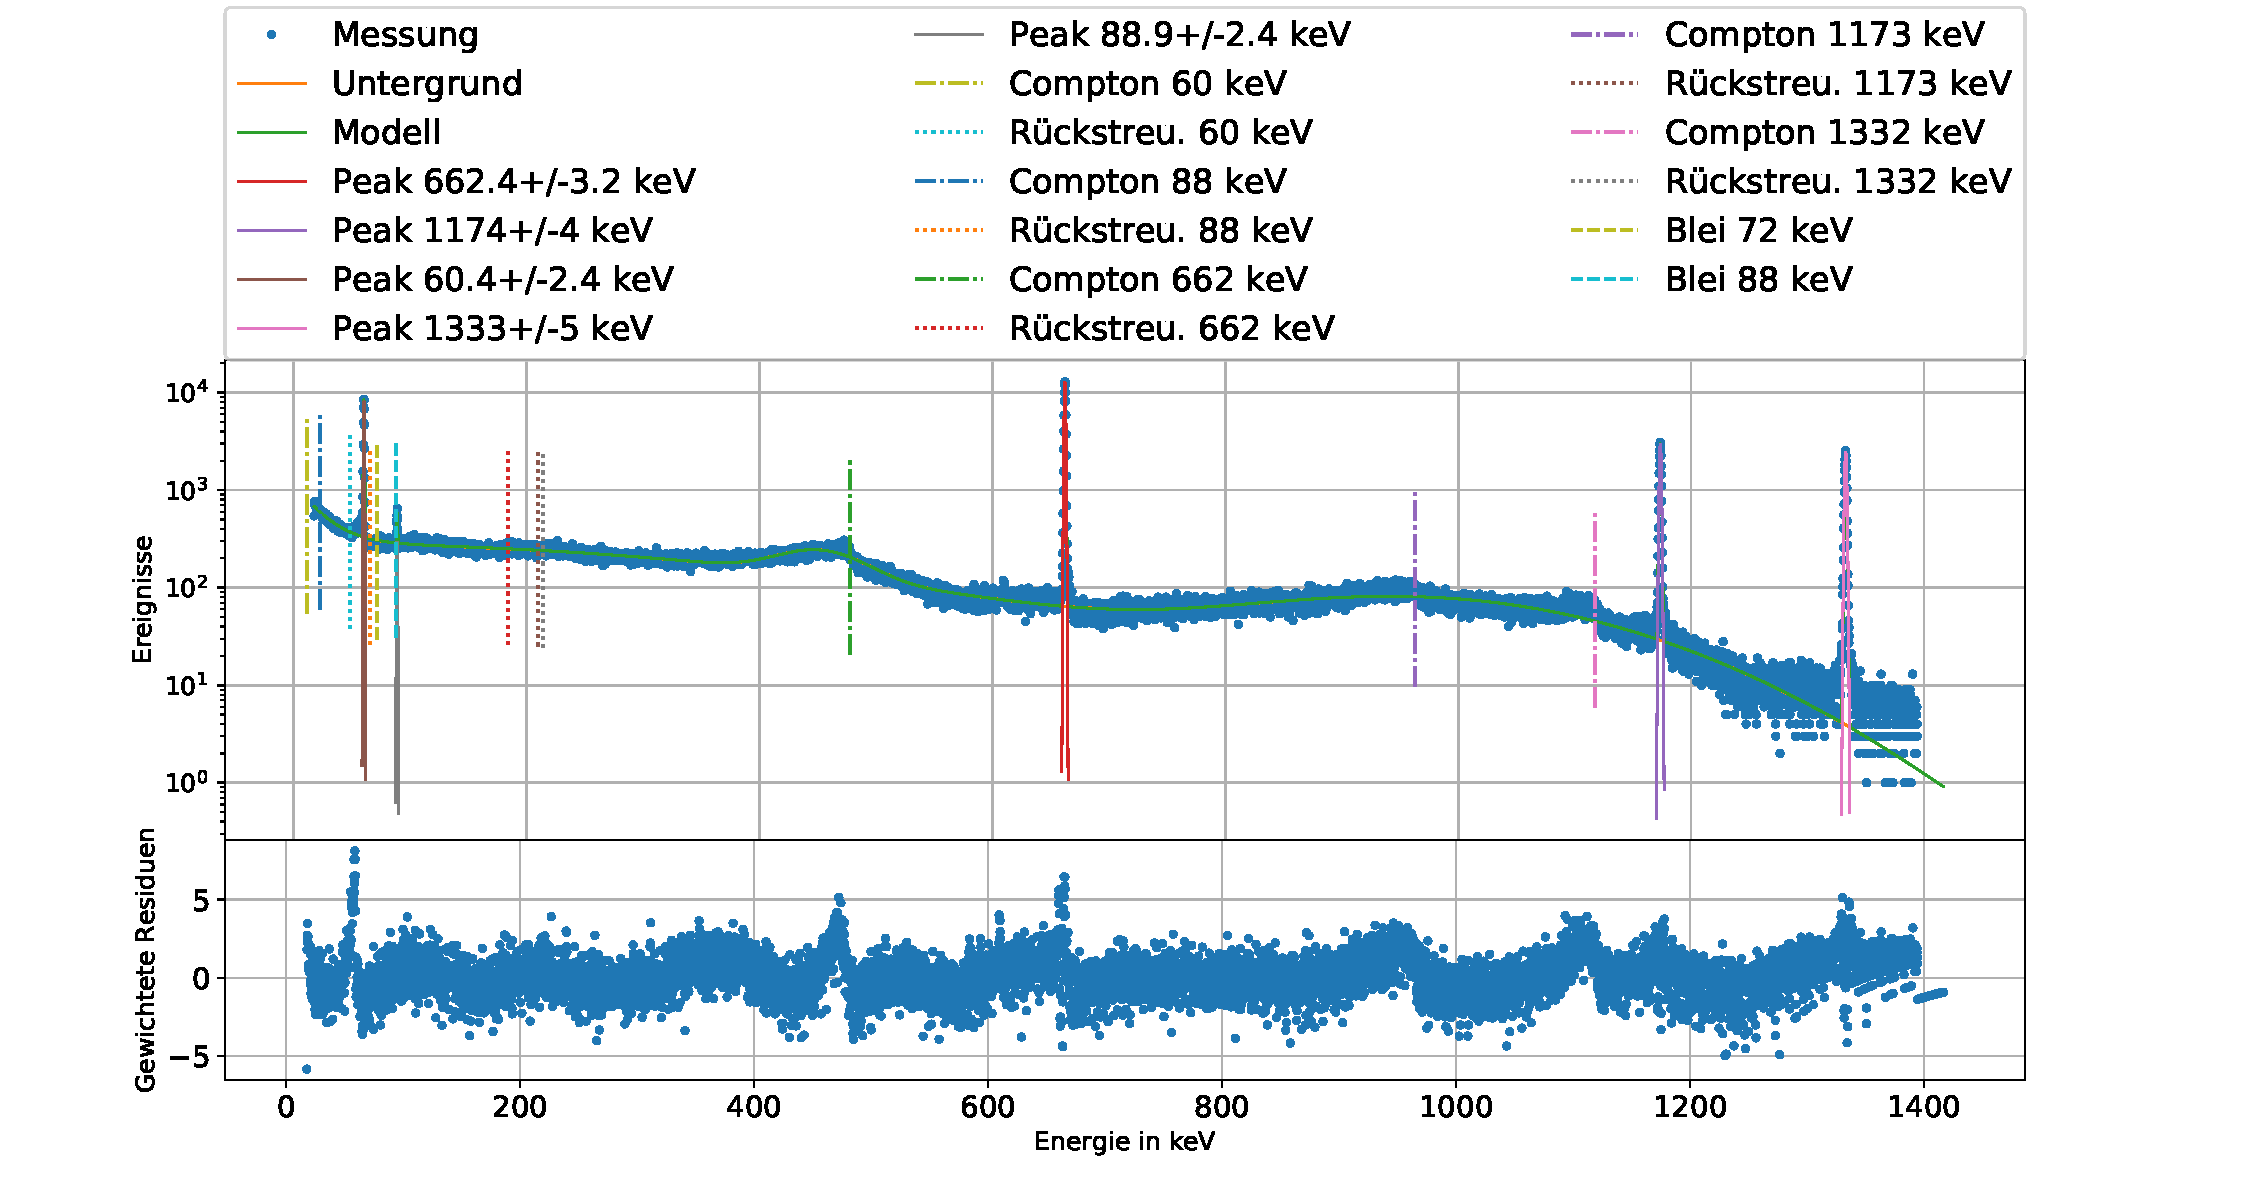
\includegraphics[width= 1 \linewidth]{img/MixGe.pdf}
			\subcaption{
				Ge-Detektor.
			}
		\label{fg_Mix_Ge}
		\end{subfigure}
		\caption{Mischprobe}
		\label{fg_Mix}
	\end{figure}
	%TODO Diskuss Anzahl Peaks verschieden => NA ist schlechter vong auflösung.

\subsection{Diskussion}

Bei der Betrachtung von \cref{fg_Na} sieht man, dass neben den Peaks anhand denen kalibriert wurde, beim NaI-Detektor auch ein Peak im Bereich der Röntgenfluoreszenz von Blei gemessen wurde.
Dieser ist im Spektrum des Ge-Detektors nicht zusehen, da hier keine Blei-Abschirmung vorhanden war.
Die Compton-Kanten und Rückstreu-Compton-Kanten sind in beiden Spektren zu erkennen (man beachte die logarithmische Skalierung, die den Abfall weniger drastisch aussehen lässt).

Auch in \cref{fg_Cs} lassen sich die Compton- und Rückstreukanten sowie der Peak durch Abregung bei \SI{662}{keV} (vgl. \cref{fig_zerfallsschemata}) erkennen.
Hier ist der Peak durch Röntgenfluoreszenz im Blei beim NaI-Detektor deutlich geringer ausgeprägt, da große Teile der Bleiabschirmung für diese Messung entfernt wurden.

In \cref{fg_Co} sieht man die gemäß \cref{fig_zerfallsschemata} erwarteten Full Energy Peaks bei \SI{1173}{keV} und \SI{1332}{keV} sowie die jeweiligen Compton- und Rückstreukanten.
Hier ist beim NaI-Detektor auch deutlich der Röntgenfluoreszenzpeak zu erkennen.

Für die Mischprobe in \cref{fg_mix} lassen sich die vielen, in die Abbildung eingezeichneten, Peaks und Kanten erkennen.
Anhand dessen konnten die in \cref{tb_lit_peaks} dargestellten Stoffe aus der Mischprobe zugeordnet werden.
Es fällt allerdings auf, dass im beim Ge-Detektor zwei Peaks bei \SI{60.4\pm 2.4}{keV} und \SI{88.9\pm 2.4}{keV} auftreten, während im NaI-Detektor nur ein Peak bei \SI{40\pm 60}{keV} gemessen wurde.
Hier ist zu vermuten, dass die einzelnen Peaks im schlechter aufgelösten NaI-Detektor zu einem einzelnen Peak verschmelzen.

Double Escape Peak oder Single Escape Peak sind nirgendwo zu sehen.
Dies bedeutet, dass die Paarbildung keinen großen Effekt im Spektrum ausmacht, da ansonsten aufgrund der hohen Reichweite der $\gamma$-Photonen in Materie einige der Photonen aus dem Detektor entkommen würden und man die verschobenen Peaks sehen würde.
Dies deckt sich mit den Erwartungen gemäß \cref{fig_wirkunsquerschnitt_gamma}, da die gemessenen Energien unter dem Einsetzen der Paarbildung liegen.

\subsection{Nichtlinearität des Detektors}
Die Nichtlinearität des Detektors kann ermittelt werden, indem man die relative Differenz der gemessenen Peaks gegen den Referenzwert des Peaks aufträgt.
Also
\begin{equation}
	\delta(E_r) = 1- \frac{E_m}{E_r}
\end{equation}
Diese Differenz wurde  in \cref{fg_diff_na} und \cref{fg_diff_ge} für NaI- und Ge-Detektor dargestellt.
$E_r$ ist Literaturwert (aus \cref{tb_lit_peaks}) für die Peakposition und $E_m$ ist der gemessenen Wert.

%TODO log plot hier von?
%TODO no errors hier?
\begin{figure}[H]
		\centering
		\begin{subfigure}[t]{0.8\textwidth}
			\centering
			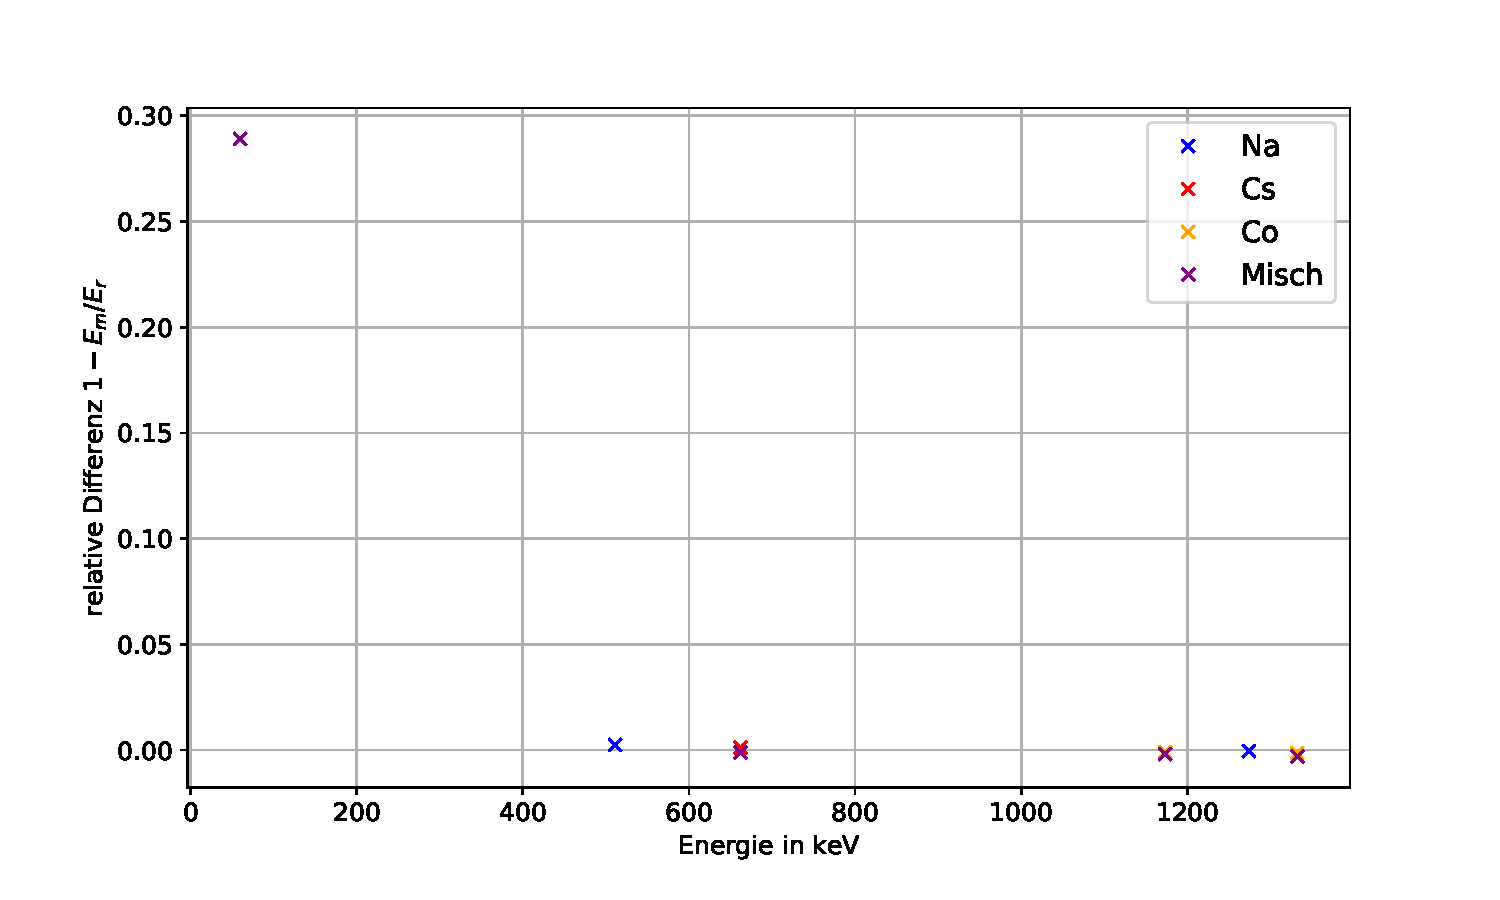
\includegraphics[width= \linewidth]{img/diff_na.pdf}
			\subcaption{
				relative Differenz.
			}
		\end{subfigure}
		\begin{subfigure}[t]{0.8\textwidth}
			\centering
			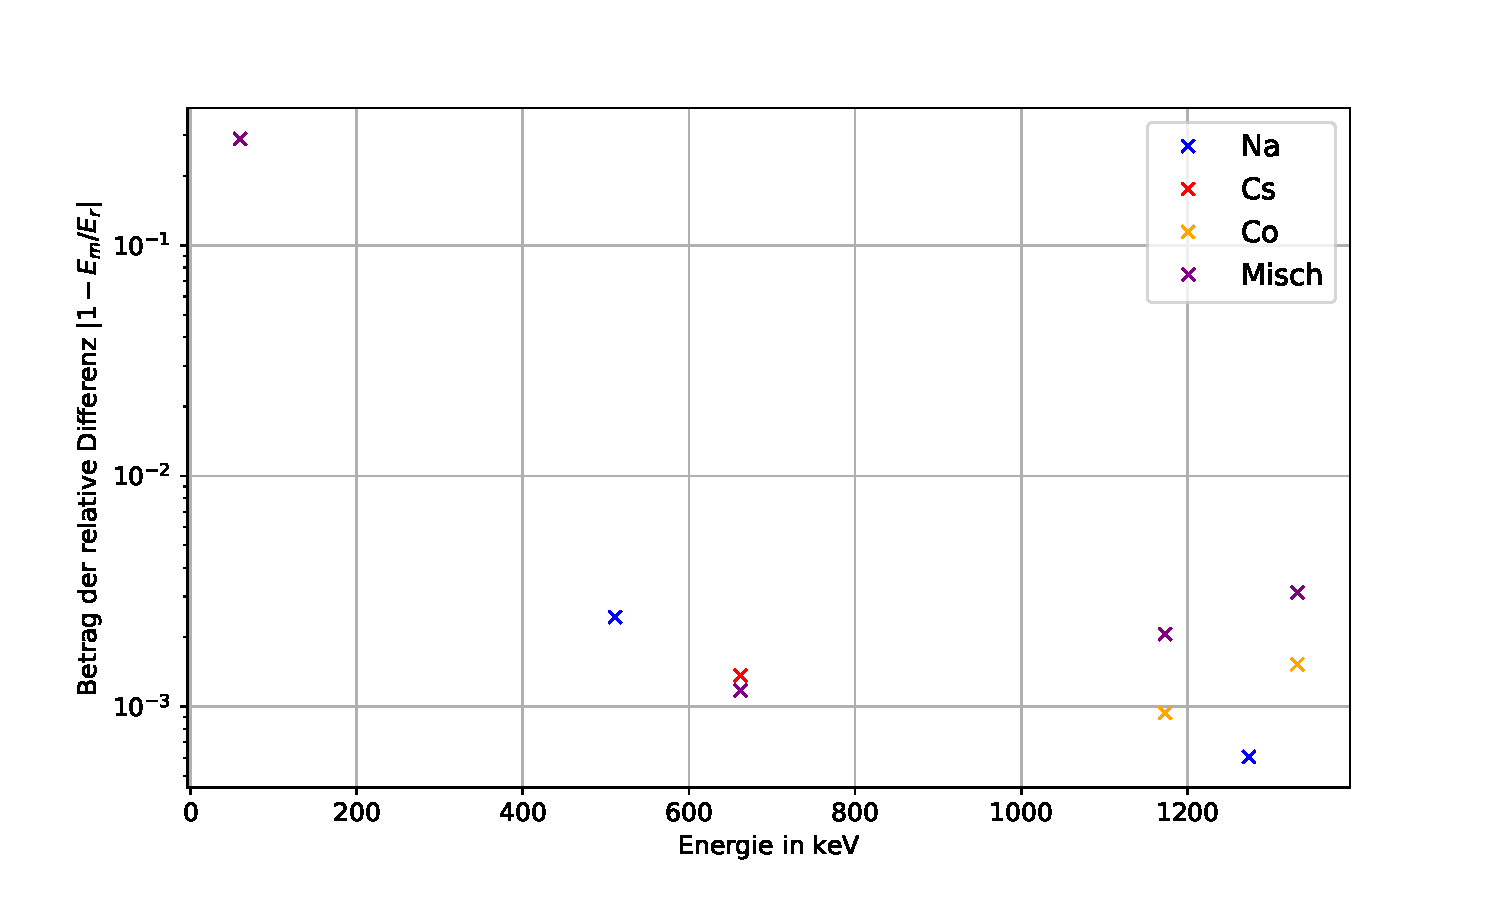
\includegraphics[width=\linewidth]{img/diff_na_log.pdf}
			\subcaption{
				Betrag der relativen Differenz in logarithmischer Darstellung.
			}
		\end{subfigure}
		\caption{Nichtlinearität des NaI-Detektors.
		Die Unsicherheiten sind nicht abgebildet, da ein Abbilden dieser ein Unterscheiden der Werte unmöglich macht. %TODO ...da sie im Vergleich sehr groß sind.
		Der Wert Null für die relative Differenz liegt immer im Unsicherheitsintervall.
		}
		\label{fg_diff_na}
	\end{figure}
\begin{figure}[H]
		\centering
		\begin{subfigure}[t]{0.8\textwidth}
			\centering
			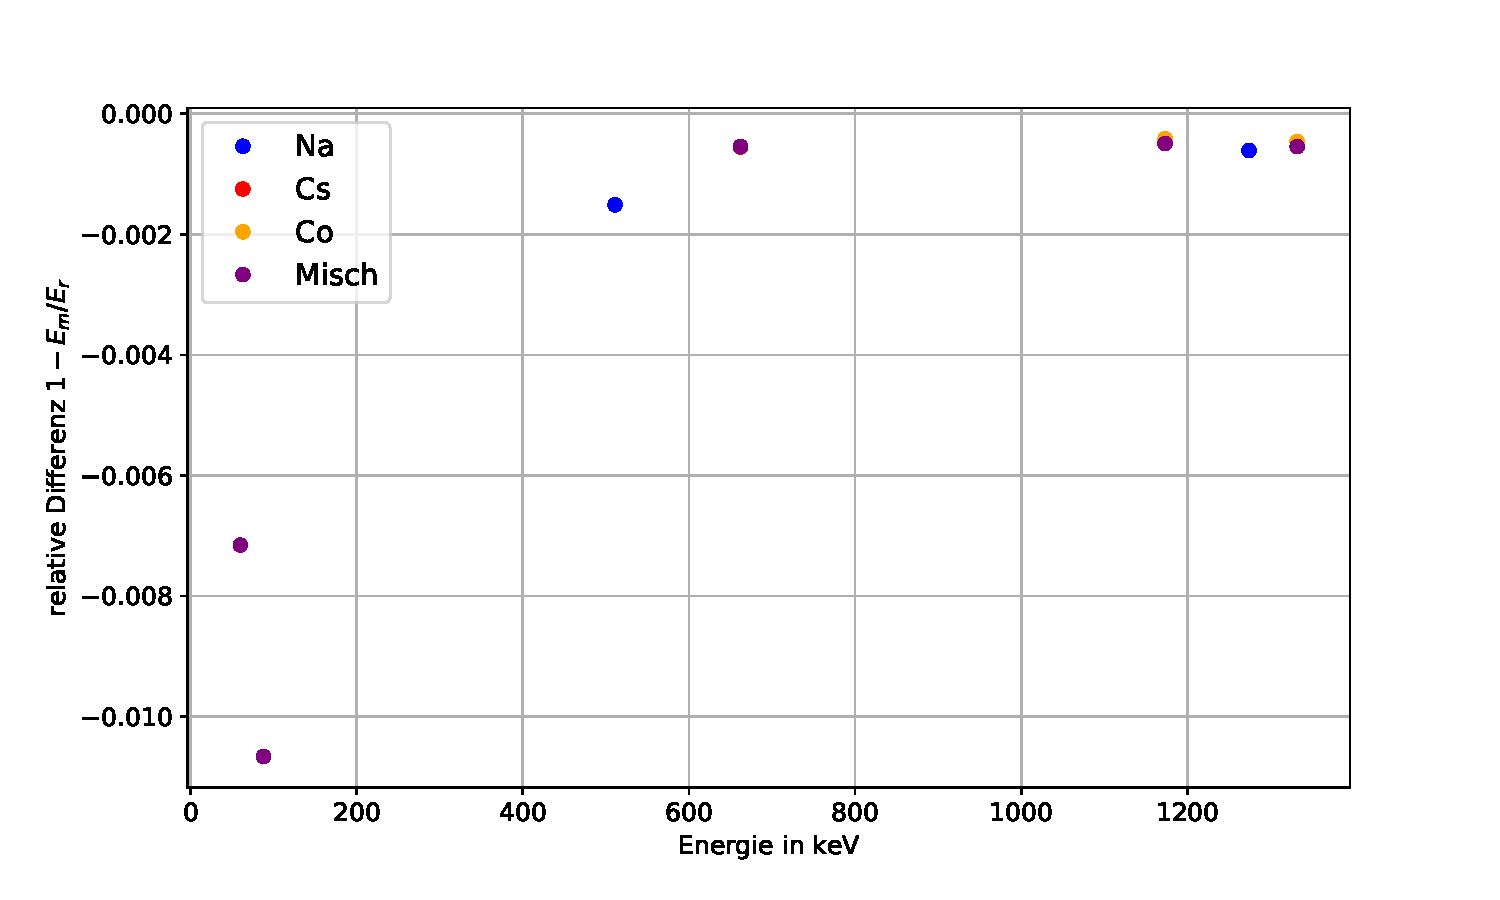
\includegraphics[width= \linewidth]{img/diff_ge.pdf}
			\subcaption{
				relative Differenz.
			}
		\end{subfigure}
		\begin{subfigure}[t]{0.8\textwidth}
			\centering
			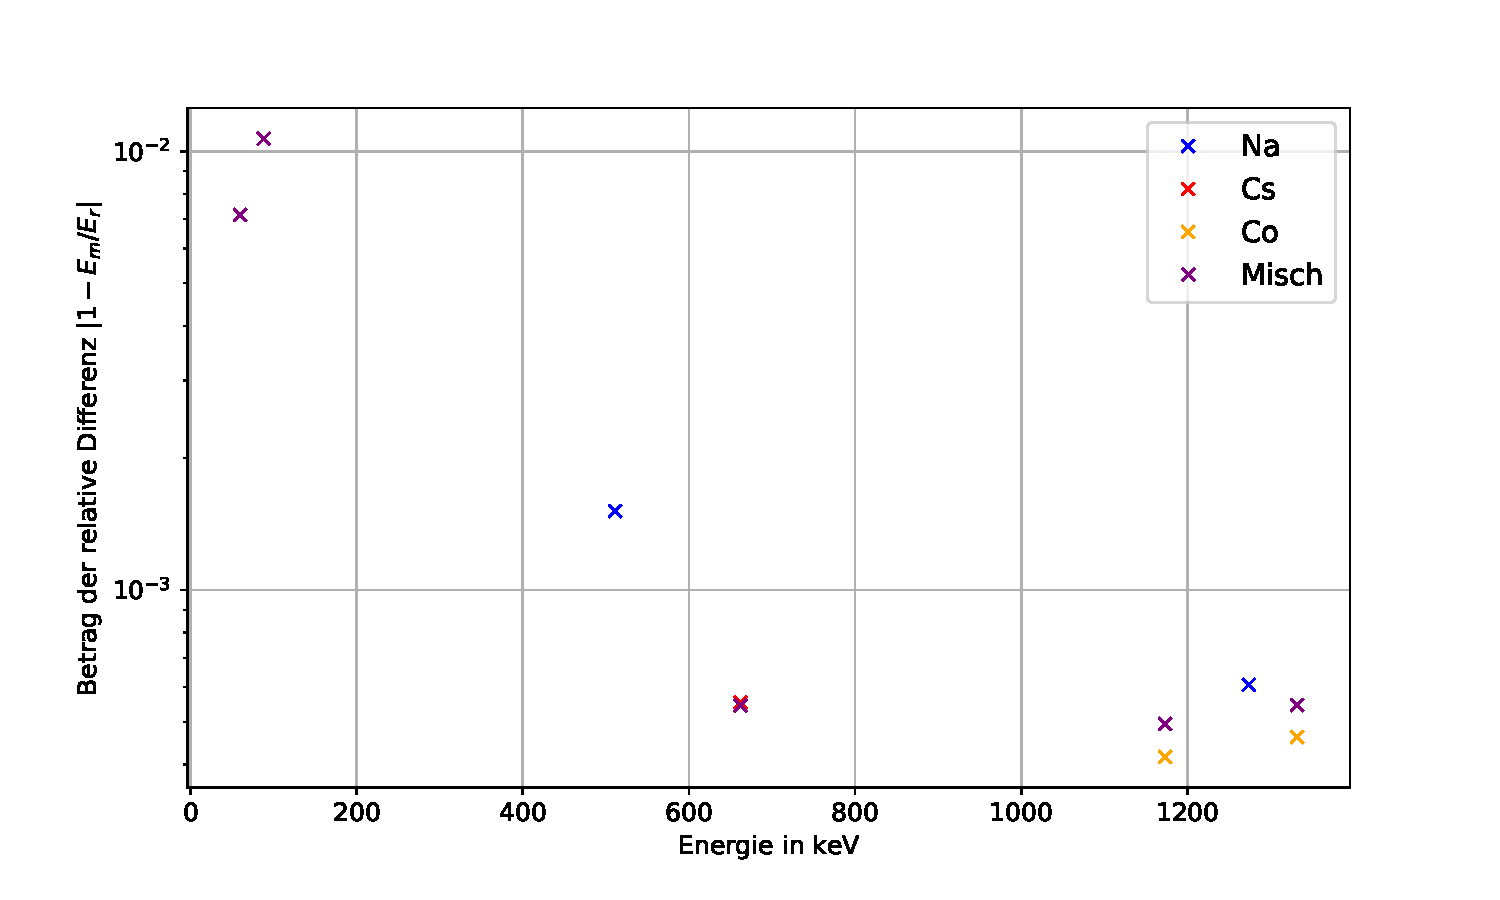
\includegraphics[width= \linewidth]{img/diff_ge_log.pdf}
			\subcaption{
				Betrag der relativen Differenz in logarithmischer Darstellung.
			}
		\end{subfigure}
		\caption{Nichtlinearität des Ge-Detektors.
		Die Unsicherheiten sind nicht abgebildet, da ein Abbilden dieser ein Unterscheiden der Werte unmöglich macht.
		Der Wert Null für die relative Differenz liegt immer im Unsicherheitsintervall.
		}
		\label{fg_diff_ge}
	\end{figure}


	\subsection{Diskussion}

	Die relative Differenz ist bei Betrachtung der logarithmischen Darstellung in \cref{fg_diff_na} für den NaI-Detektor bei geringen Energien am höchsten und steigt auch für sehr hohe Energien leicht.
	Beim Ge-Detektor in \cref{fg_diff_ge} ist dieser Zusammenhang ähnlich.
	Dies zeigt, dass beide Detektoren nicht exakt linear Photonenenergie in Signalspannung und dann in Kanalnummer umsetzen.

\subsection{Energieauflösung}
Die Energieauflösung $\Delta E$ lässt sich aus der Standardabweichung $\sigma$ und der Position $E$ eines Full-Energy-Peaks berechnen.
Die Formel hierfür ist:
\begin{equation}
	\Delta E = \frac{\sigma}{E}
\end{equation}
Die Unsicherheiten für $\sigma$ ergeben sich aus der Multiplikation mit der Steigung $m$ aus der Kalibrationsgeradengleichung (\ref{eq_trans}).


	\begin{figure}[H]
			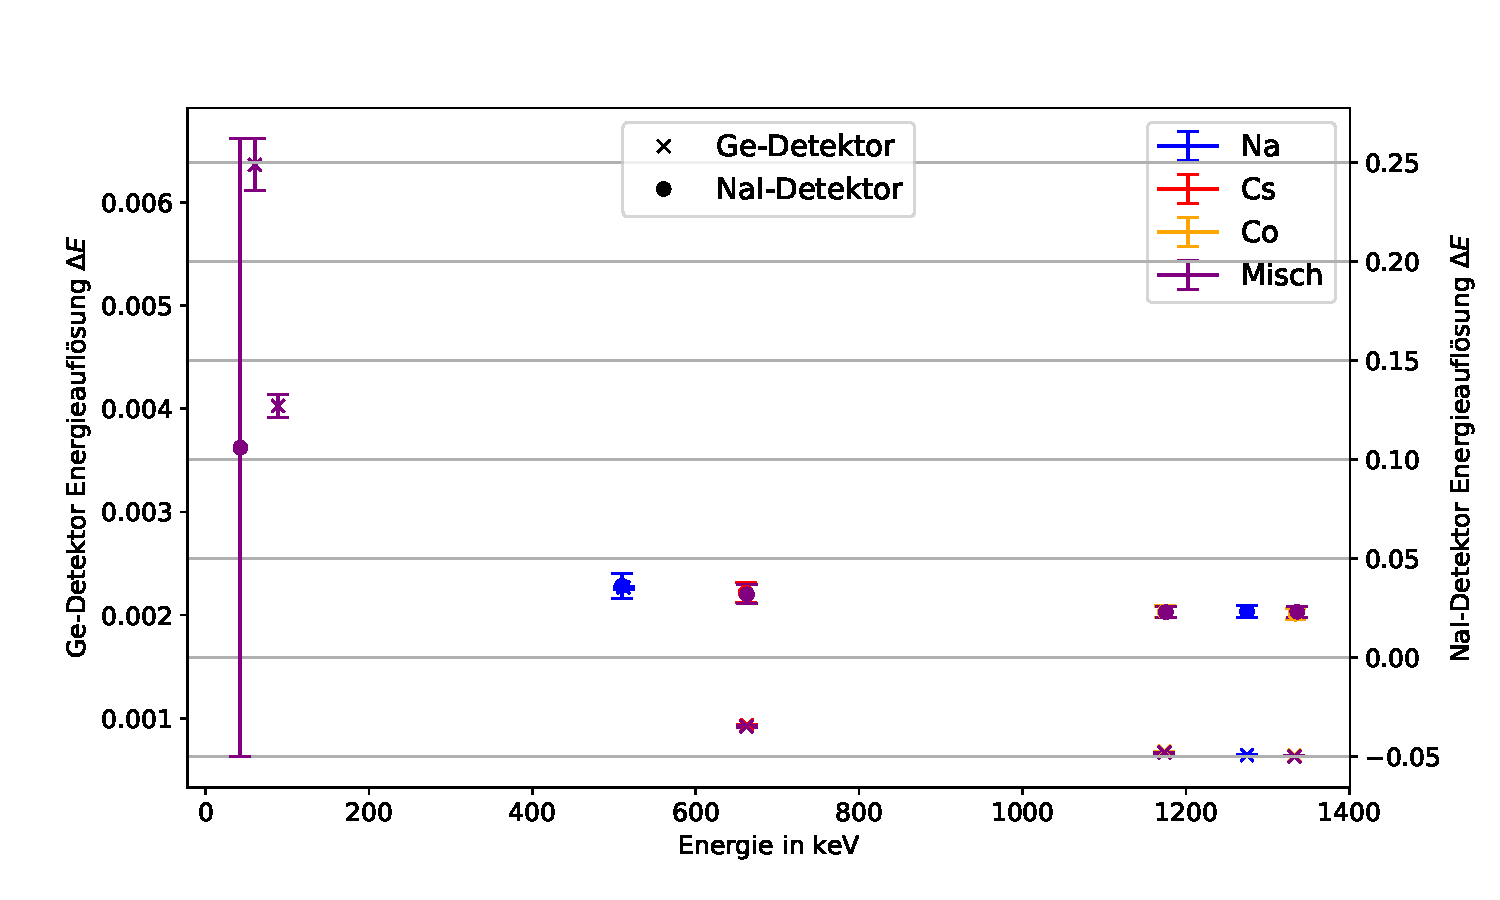
\includegraphics[width= 1 \linewidth]{img/res}
			\caption{
			Energieauflösung für NaI- und Ge-Detektor.
			}
			\label{fg_resolution}
	\end{figure}


\subsection{Diskussion}

Die große Unsicherheit des niederenergetischen NaI-Detektor Messpunkts ist der großen (relativen) Unsicherheit des ersten Peaks in der Mischprobe geschuldet (\cref{fg_Mix_Na}).
Es lässt sich erkennen, dass die Energieauflösung für beide Detektoren zu hohen Energien hin abnimmt.
Außerdem ist die Auflösung des NaI-Detektors immer höher, wie bereits zuvor anhand der großen Peakbreite angemerkt wurde, weshalb hier der Ge-Detektor zu bevorzugen ist.

\subsection{Mittlere Ionisationsenergie}
Die Mittlere Ionisationsenergie $I$ lässt sich ebenso aus der Standardabweichung $\sigma$ und der Position $E$ eines Full-Energy-Peaks berechnen.
Die Formel hierfür ist:
%TODO Theo: explain calc
\begin{equation}
	I = \frac{\sigma^2}{E}
\end{equation}
Die Unsicherheiten für $\sigma$ ergeben sich aus der Multiplikation mit der Steigung $m$ aus der Kalibrationsgeradengleichung (\ref{eq_trans}).
In \cref{fg_ionisation} ist $I$ für beide Detektoren gegen $E$ aufgetragen.


	\begin{figure}[H]
			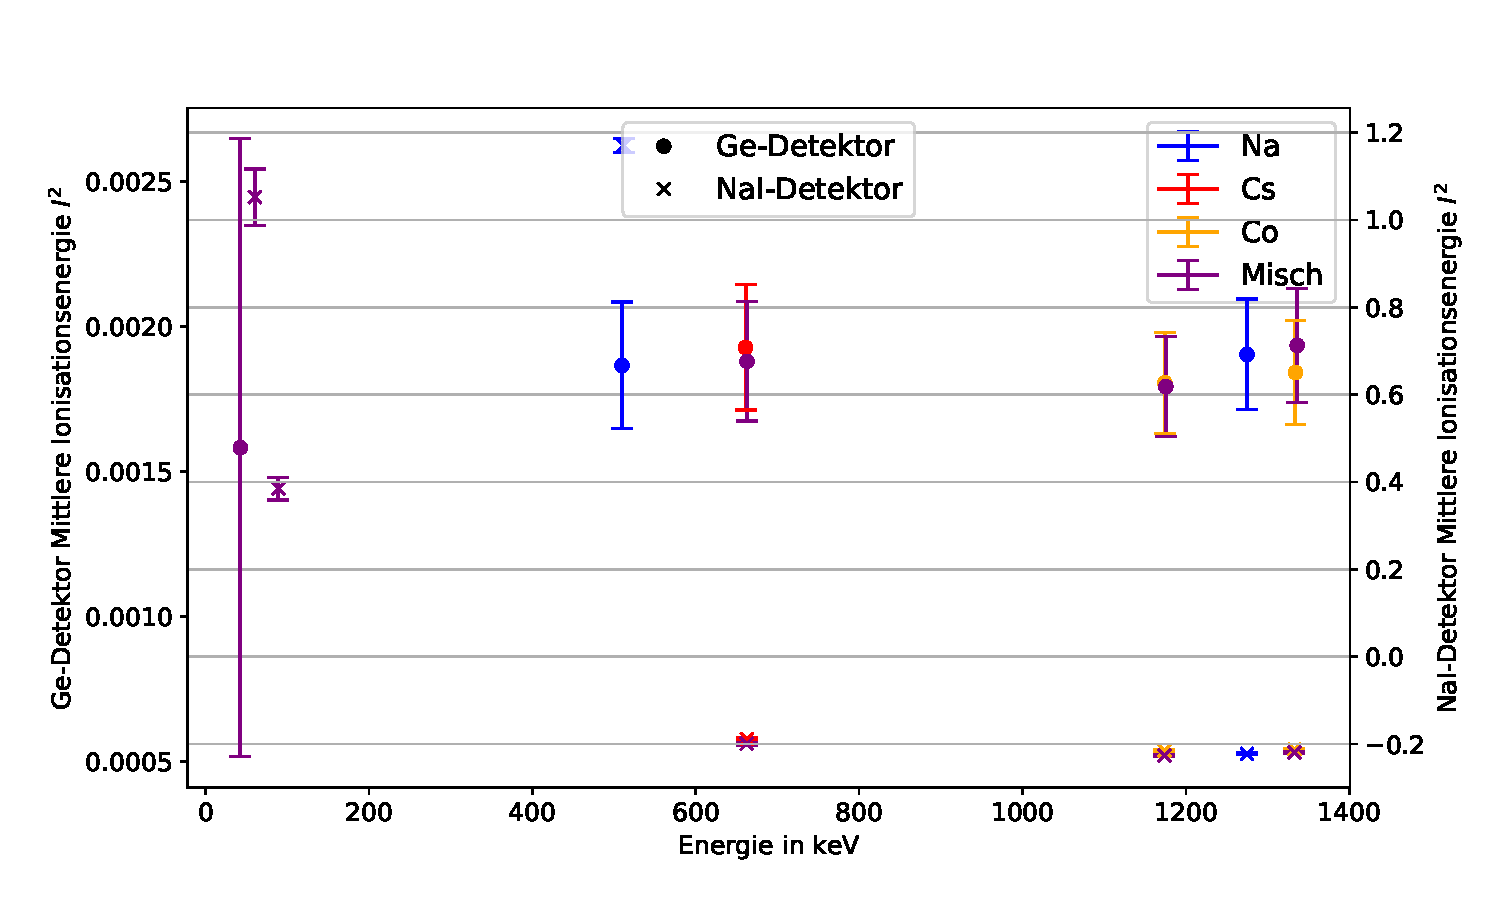
\includegraphics[width= 1 \linewidth]{img/ion}
			\caption{
			Mittlere Ionisationsenergie für NaI- und Ge-Detektor.
			}
			\label{fg_ionisation}
	\end{figure}

%\subsubsection{Diskussion}

Die mittlere Ionisationsenergie des Ge-Detektors ist im Allgeimeinen deutlich geringer als die des NaI-Detektors. %TODO mehr weiß ich net.

\subsection{Relative Effizienz}
Die relative normierte Effizienz $\varepsilon$ lässt sich nach \cref{eq_rel_eff} berechnen.
\begin{equation}
	\label{eq_rel_eff}
	\varepsilon = \frac{\frac{S}{P}}{\left|\frac{S}{P}\right|}_{\text{ref}}
\end{equation}
%TODO in Theorie: Full Energy Peak ETC.
Wobei $S$ die Fläche eines Full-Energy-Peaks ist und $P$ die Anzahl Photonen, welche im Messzeitraum $t$ durch diesen $\gamma$-Übergang ausgesendet werden.
Dieses Verhältnis wird auf einen Messpunkt $\left|\frac{S}{P}\right|_{\text{ref}}$ normiert.
Die Anzahl Photonen ist das Produkt aus Messdauer $t$ und Aktivität $A$ des $\gamma$-Übergangs, $P=A\cdot t$.
Die derzeitige ($t'$) Aktivitäten wurden aus einer vorherigen ($t_r$) Messung und bekannter Zerfallskonstante $\lambda$ berechnet.
\begin{equation}
	A(t') = A(t_r)\exp^{-\lambda (t'-t_r)}
\end{equation}
Die Ergebnisse sind in \cref{fg_eff} gegen die Energie $E$ aufgetragen.
Als Normierung wurde für beide Detektoren der Full-Energy-Peak bei \SI{662}{keV} verwendet.

	\begin{figure}[H]
			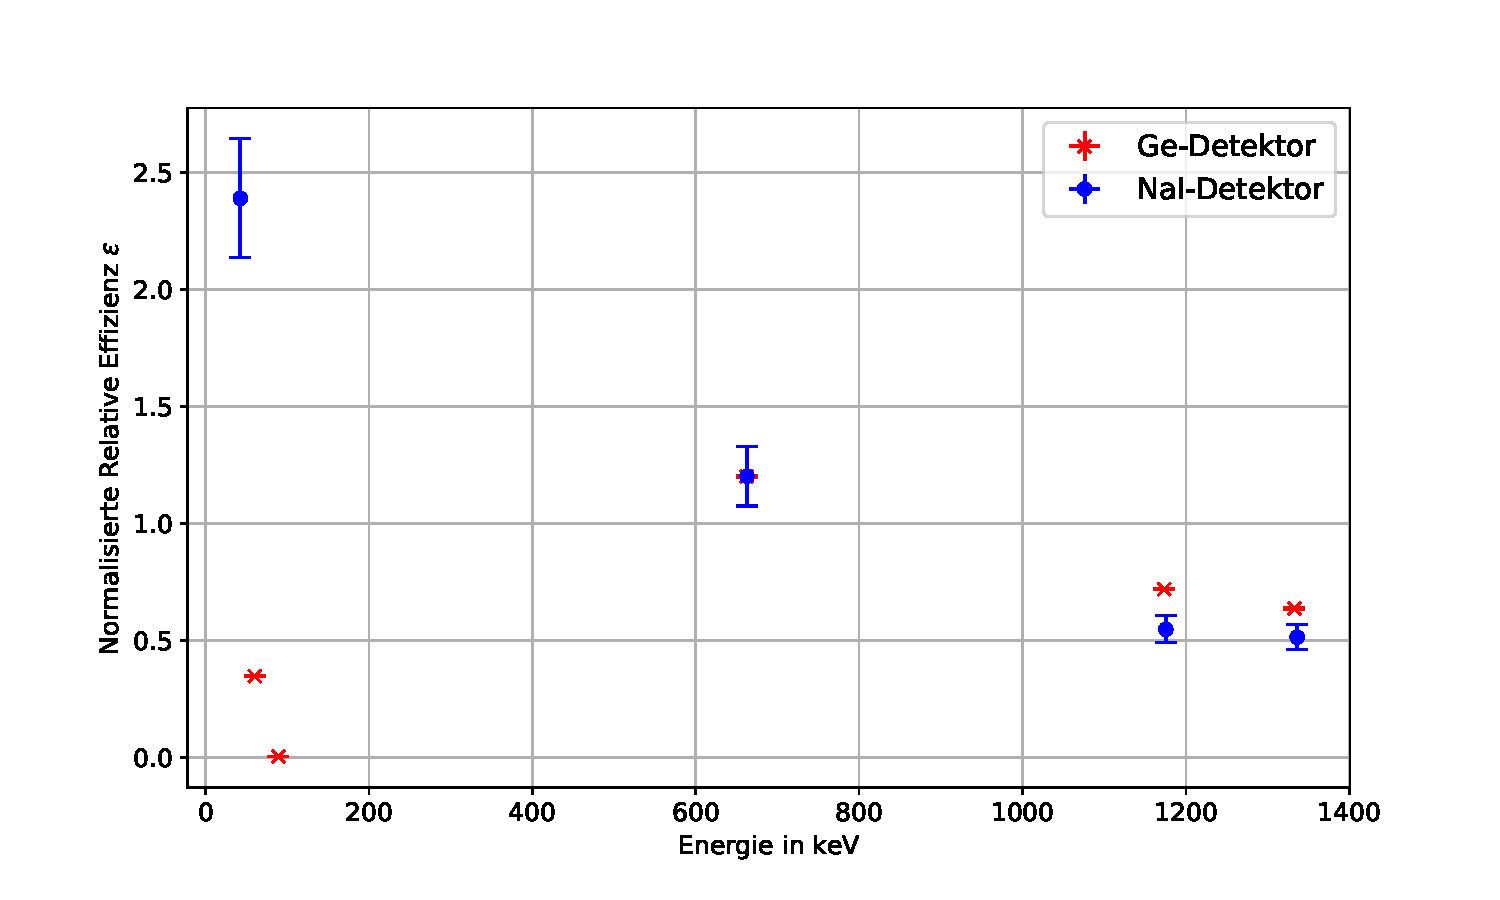
\includegraphics[width= 1 \linewidth]{img/eff}
			\caption{
			Normierte Relative Effizienz für NaI- und Ge-Detektor bei der Mischprobe.
			}
			\label{fg_eff}
	\end{figure}
	% Diskuss: grund für hohe NaI-Wert: Auflösung zuschlecht für die zwei peaks die Ge da hat, stackt sich dann.

\subsubsection{Diskussion}

In \cref{fg_eff} ist zu erkennen, dass für den NaI-Detektor die normierte relative Effizienz mit der Energie abnimmt, während für den Ge-Detektor kein Zusammenhang erkannt werden kann.
Bis auf den ersten Messpunkt ist die Effizienz des Ge-Detektors aber gleich hoch oder höher.
Der erste Messpunkt ist auf die Überlagerung von zwei Peaks infolge der schlechten Auflösung dieses Detektors zurückzuführen.
Um möglichst viele Photonen nachzuweisen, ist mit dem verwendeten Aufbau der Ge-Detektor vorzuziehen.
Faktisch hängt hier natürlich die Effizienz vorallem von der Raumgeometrie ab, weshalb hier ein direkter Vergleich nicht möglich ist.

\subsection{Erzprobe}
	In \cref{fg_erz} ist das Spektrum der Erzprobe abgebildet.
	In unterschiedlichen Farben sind die am deutlichsten passenden Peaks der vier natürlichen Zerfallsreihen markiert.
	Im \nameref{s_anhang} sind in \crefrange{fg_erz_np}{fg_erz_u_ra} die Zerfallsreihen separat markiert.
	Hierbei wurde nach Augemaß Schwarz für einen passenden Peak, Rot für einen verschobenen oder schwachen Peak, und Blau für keine Korrelation verwendet.
	Die Literaturwerte für die Energien $E_\gamma$ stammen aus \cite{erze1} und \cite{erze2}.
	Es wurden direkt Peaks mit einer relativen Intensität kleiner als \SI{5}{\percent} ausgeschlossen.

	\begin{figure}[H]
			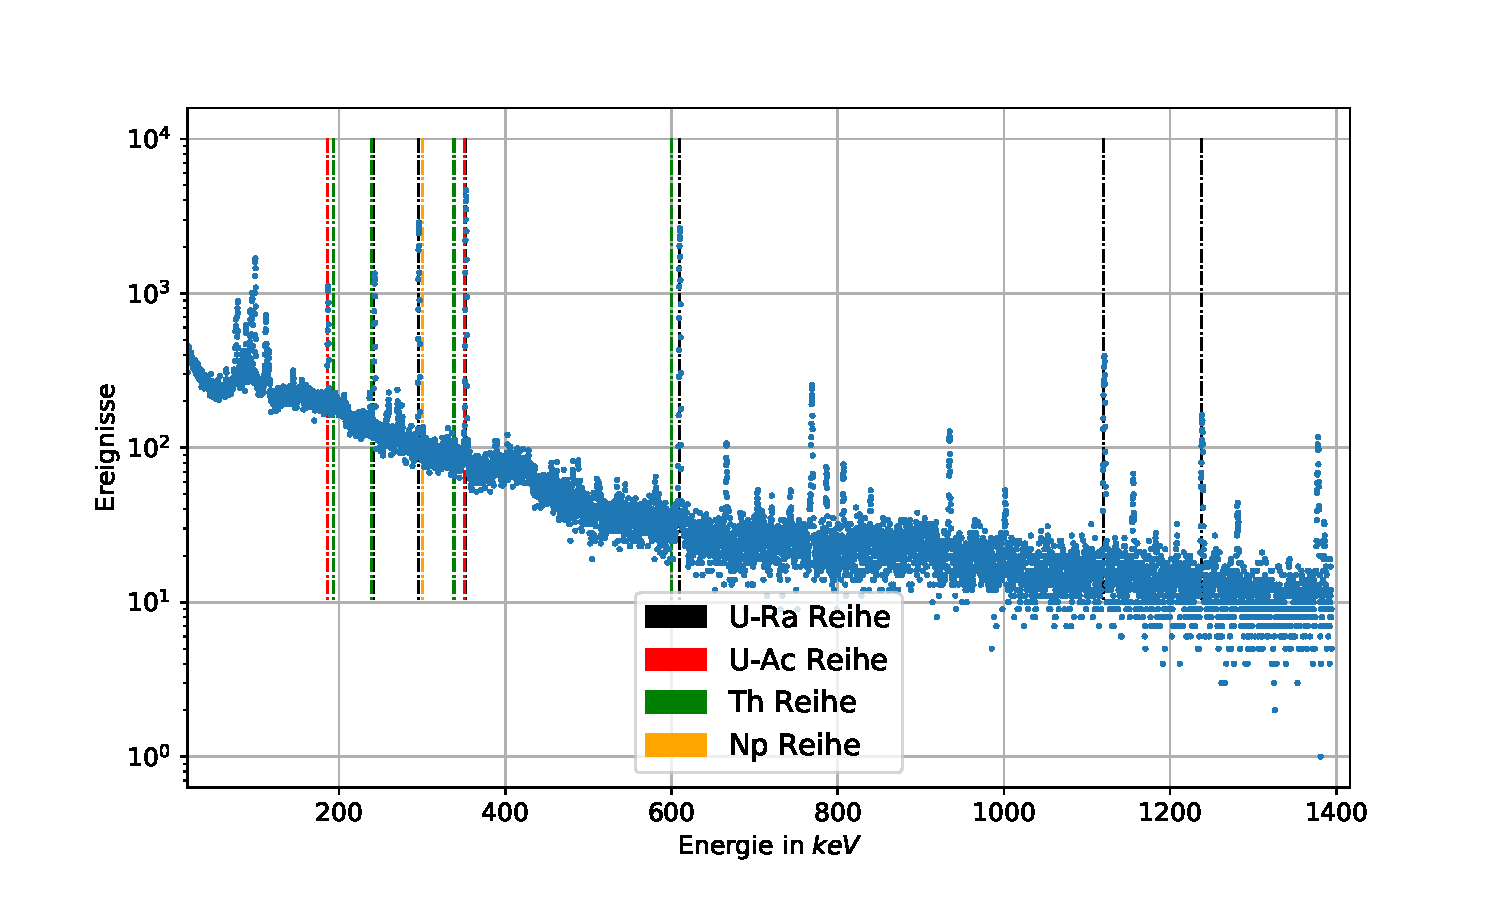
\includegraphics[width= 1 \linewidth]{img/erz_alles}
			\caption{
			Spektrum der Erzprobe. Einige passende $\gamma$-Übergangenergien sind von den vier Zerfallsreihen farblich eingezeichnet. Verwendet wurde der Ge-Detektor.
			}
			\label{fg_erz}
	\end{figure}

\subsubsection{Diskussion}

	Besonders gut zu erkennen sind $^214$Pb und $^214$Bi.
	Anhand der Zerfallsreihen lässt sich damit die Probe der Uran-Radium-Reihe zuordnen, weshalb es sich bei dem Erz wohl ursprünglich um $^238$U handelte. %TODO kann man das so sagen?
	% Bezug/Nutzen oder sonst was
	% auch hier die Hypothese wiederholen
	% keine Messwerte hier, nach manchen Menschen, zumindest "direkt" erstellte Diagramme net hier, auch wenn Lesbarkeit-bla
	% Rückstreuungsminimierung durch Deckel abnehmen aber immernoch Luft/Decke/we

	%\subsection{Interpretation}
	% features of typical gamma spectrum
	% Vergleich Literaturwerte der gammalinien
	% Vergleich Literaturwerte der comptonkanten
	% zusätzliche Peaks zusehen?
	% welche der erwarteten Peaks in der Mischprobe?
	% welche Isotope in der unbekannten Probe? Zu welcher Zerfallsreihe gehören die.

	%\subsection{Vergleich der Detektoren}
	% Wie Energieunschärfe?
	% Zusammenhang Energieauflösung und mittlere Ionisationsenergie?
	% Abhängigkeit der beiden von Energie?
	% Definition der Effizienz? Wie misst man das?
	% Ist es möglich die Effizienzen zu vergleichen?->Raumgeometrie?
	% Wo sind die Detektoren ähnlich?


	%TODO warum 511 nur bei NA?
	\section{Schlussfolgerung}
	% Rückgriff auf Hypothese und drittes Nennen dieser
	Insgesamt gesehen lässt sich sagen, dass alle Messungen erfolgreich durchgeführt werden konnten und die in den Spektren gemessenen Peaks den Literaturwerten zugeordnet werden konnten.
	Der Vergleich der beiden Detektoren erlaubt auch einige Aussagen bezüglich ihrer Güte zu treffen.
	Bezüglich der Energieauflösung verhält sich der Ge-Detektor deutlich besser als der NaI-Detektor, sorgt also für deutlich schärfere Peaks.
	Die Nichtlinearität der beiden Detektoren ist für den größten Teil des Spektrums etwa gleich.
	Die Nichtlinearität des Ge-Detektors ist jedoch im Allgemeinen etwas geringer.
	In Bezug auf die relative Effizienz lässt sich aufgrund mangelnder vergleichbarer Versuchsbedingungen keine vergleichende Aussage möglich.
	Hierfür müsste ein Versuch durchgeführt werden, bei dem beide Absorber den gleichen Raumwinkel in gleichem Abstand von der Probe einnehmen.

	Die Erzprobe konnte einer Zerfallsreihe zugeordnet werden.
	%TODO Ergibnis Spektren-Aussehen
	%TODO Ergebnis Vergleich detektroen
	%TODO Ergebnis unbektannte Probe


	\section{Anhang} \label{s_anhang}

	\begin{figure}[H]
			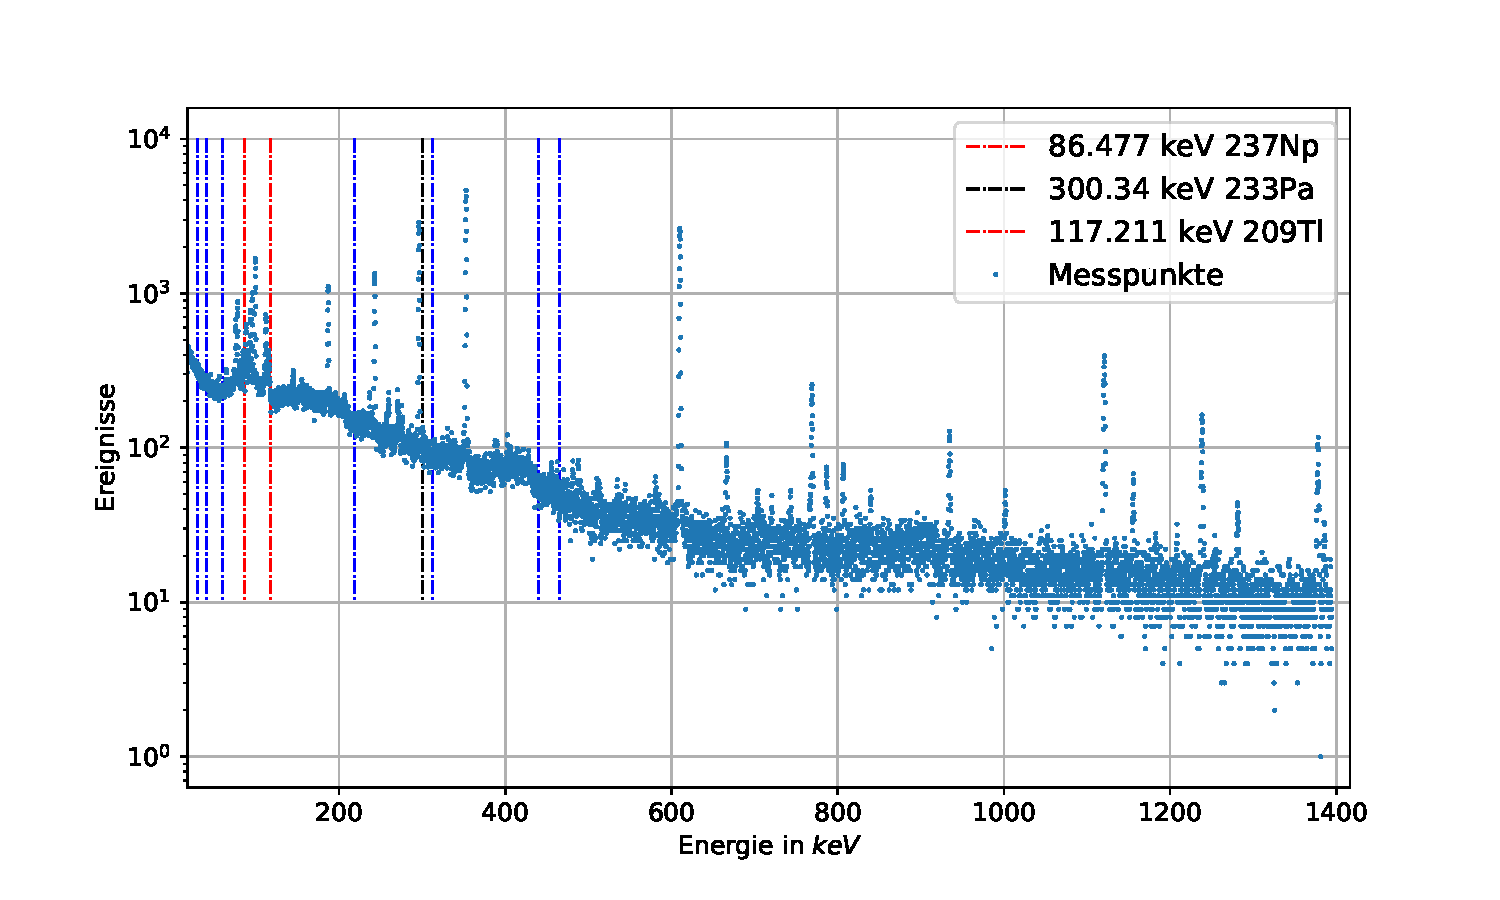
\includegraphics[width= 1 \linewidth]{img/erz_Np}
			\caption{
			Spektrum der Erzprobe. Np-Reihen $\gamma$-Übergangenergien sind von den vier Zerfallsreihen farblich eingezeichnet.
			}
			\label{fg_erz_np}
	\end{figure}
	\begin{figure}[H]
			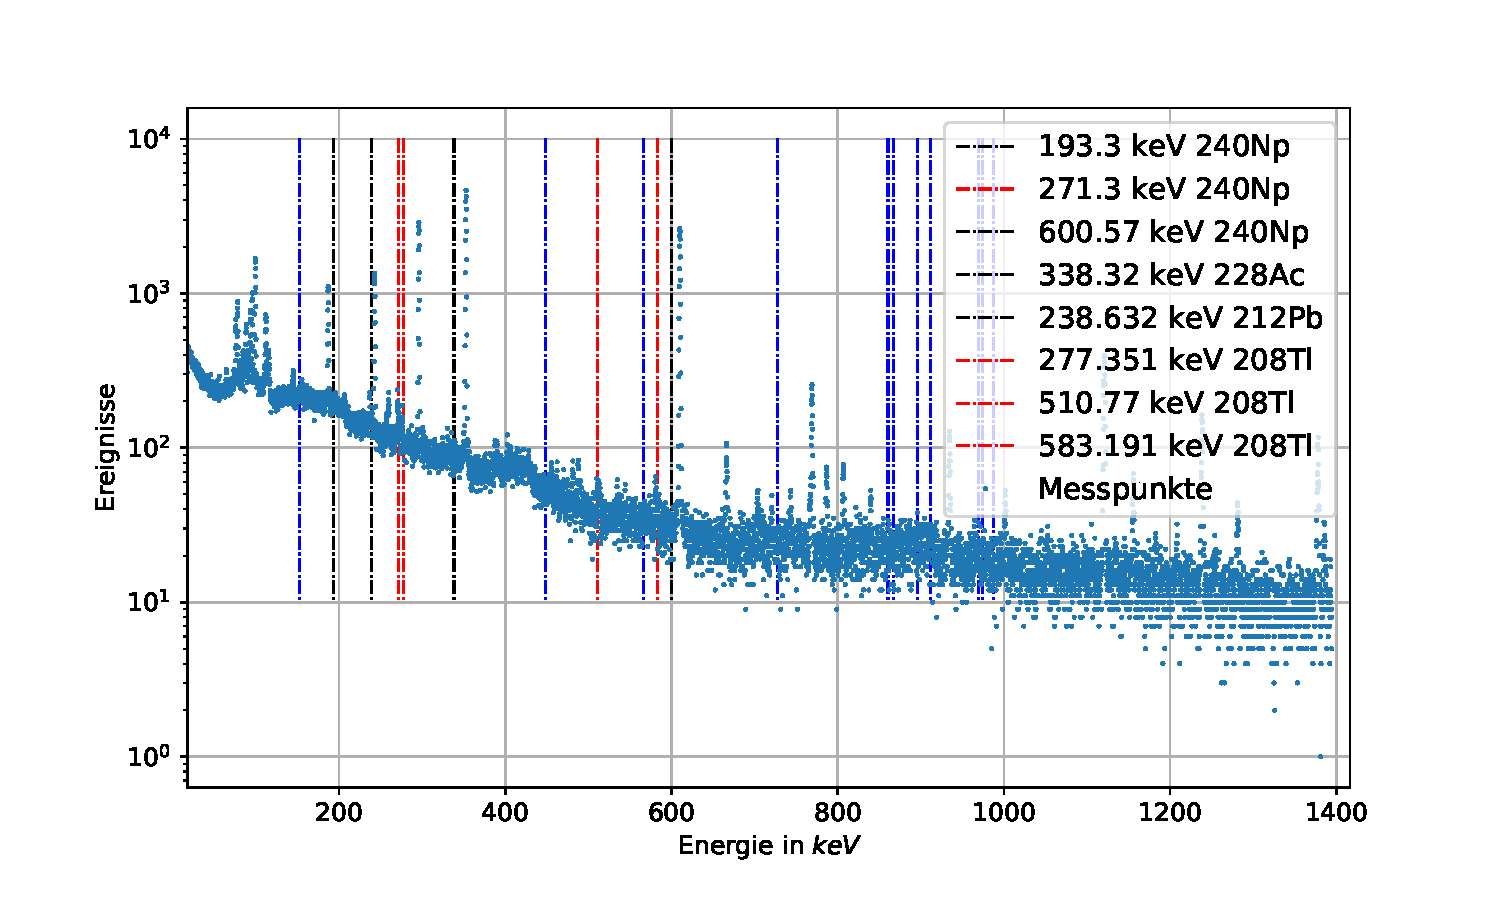
\includegraphics[width= 1 \linewidth]{img/erz_Th}
			\caption{
			Spektrum der Erzprobe. Th-Reihen $\gamma$-Übergangenergien sind von den vier Zerfallsreihen farblich eingezeichnet.
			}
			\label{fg_erz_th}
	\end{figure}
	\begin{figure}[H]
			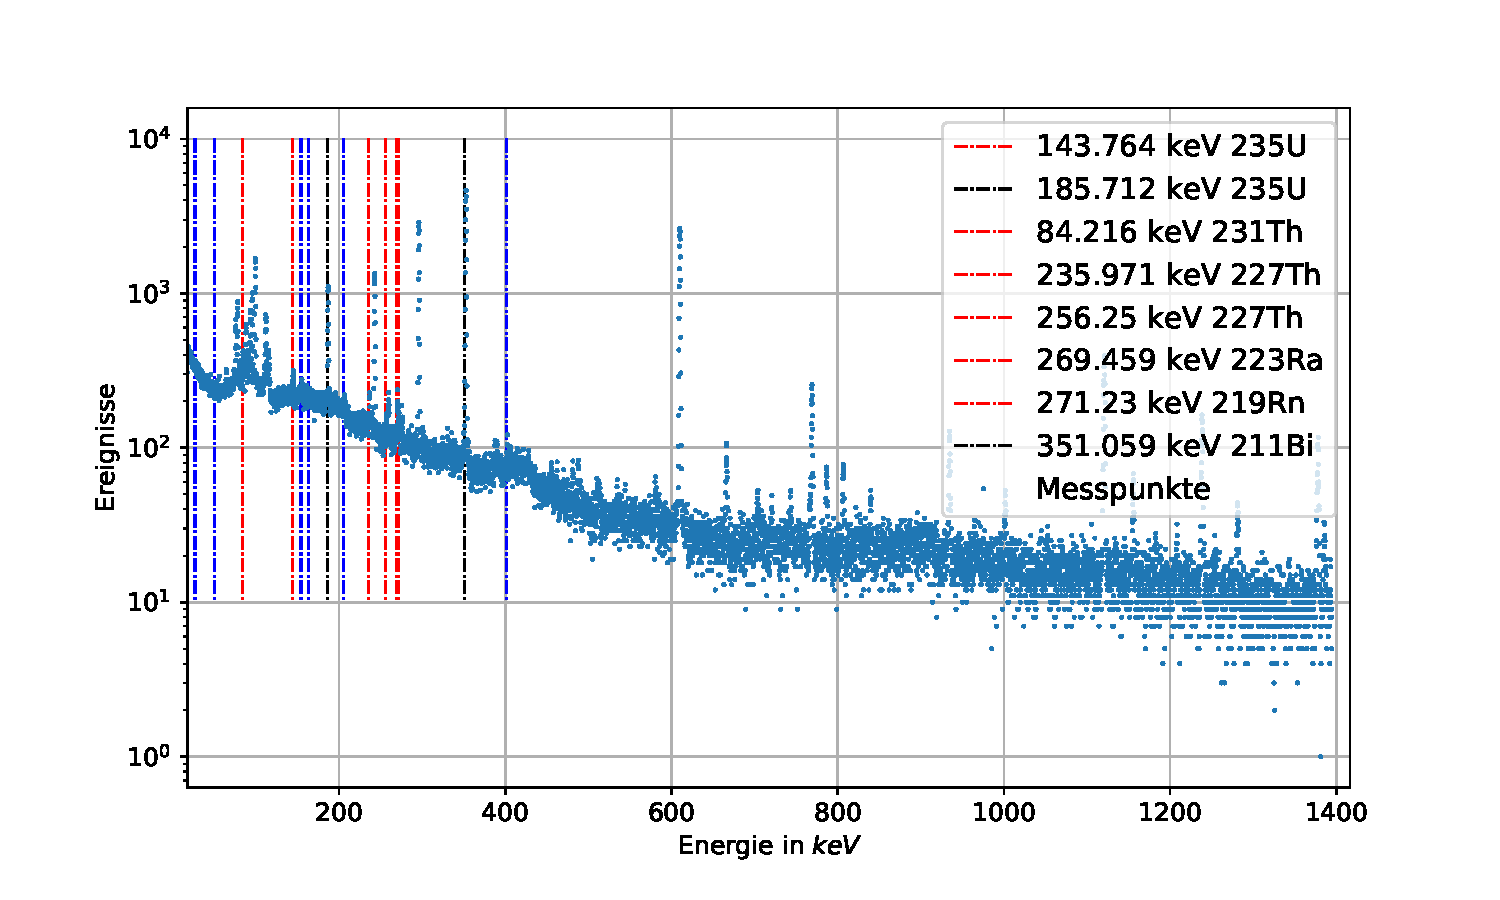
\includegraphics[width= 1 \linewidth]{img/erz_U-Ac}
			\caption{
			Spektrum der Erzprobe. $^{235}$U-Reihen $\gamma$-Übergangenergien sind von den vier Zerfallsreihen farblich eingezeichnet.
			}
			\label{fg_erz_u_ac}
	\end{figure}
	\begin{figure}[H]
			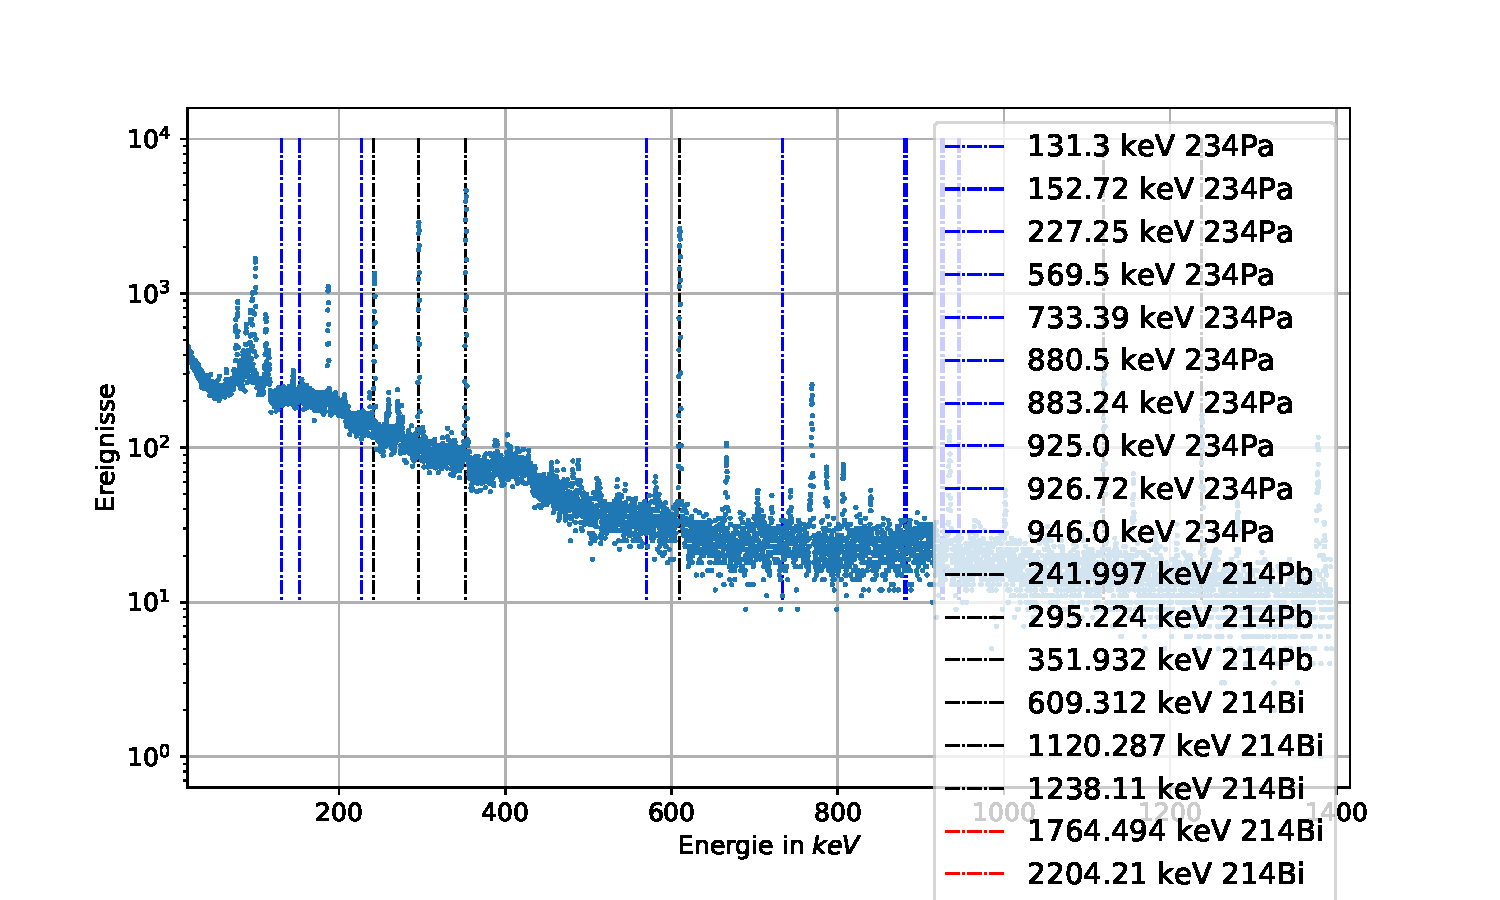
\includegraphics[width= 1 \linewidth]{img/erz_U-Ra}
			\caption{
			Spektrum der Erzprobe. $^{238}$U-Reihen $\gamma$-Übergangenergien sind von den vier Zerfallsreihen farblich eingezeichnet.
			}
			\label{fg_erz_u_ra}
	\end{figure}
	% Quellen zitieren, Websiten mit Zugriffsdatum
	% Verweise auf das Laborbuch (sind erlaubt)
	% Tabelle + Bilder mit Beschriftung
	\printbibliography
\end{document}

%TODO Ich hab der anleitung nen Datum gegeben, weil dass da drauf steht. Vielleicht ist nur das Jahr sinnvoller, weil mans bei veröffentlichungen so machen würde.
